% update 17/04/2026
\documentclass[journal]{IEEEtran}
\usepackage{cite}
\usepackage{amsmath,amsfonts,amssymb}
\usepackage{graphicx,caption}
\usepackage{epstopdf}
\usepackage{subcaption}
\usepackage{url}
\usepackage{color}
\usepackage{colortbl}
\usepackage{multirow}
\usepackage{bm}
\usepackage{algorithm}
\usepackage{algpseudocode}
\usepackage{booktabs}
\usepackage[table,xcdraw]{xcolor}
\usepackage{booktabs}
\usepackage{tabularx}
\usepackage{array}
\newcolumntype{L}{>{\raggedright\arraybackslash}X}
\usepackage[caption=false,font=footnotesize]{subfig}

\newcommand{\SNR}{\mathsf{SNR}}
\newcommand{\INR}{\mathsf{INR}}
\newcommand{\E}{\mathbb{E}}
\newcommand{\Var}{\mathrm{Var}}
\newcommand{\Cov}{\mathrm{Cov}}
\newcommand{\sym}{\mathrm{sym}}
\newcommand{\conv}{\mathrm{conv}}
\newcommand{\jg}{\mathrm{J.G.}}
\newcommand{\rank}{\mathrm{rank}}
\newcommand{\Id}{\mathbf{I}}
\newcommand{\Zero}{\mathbf{0}}
\newcommand{\figref}[1]{Fig.~\ref{#1}}
\newcommand{\tabref}[1]{Table~\ref{#1}}

\title{An EDLines-Based Virtual Encoder with Pose Estimation
for XY-Axis Calibration of a Cartesian 3D Printer}

\author{
Zayd Zihni Zaidan,~\IEEEmembership{Member,~IEEE},
Sylmina Dalily Alkaff,
Aqilah Baseri Huddin,
Hanim Hussin,
Asif Ali Zamzami,~\IEEEmembership{Member,~IEEE}
and Bahrudin
%
\thanks{Manuscript received xxx; revised xxx; accepted xxx. Date of publication xxx; date of current version xxx. (\textit{Corresponding author: Asif Ali Zamzami.})}
%
\thanks{Zayd Zihni Zaidan, Sylmina Dalily Alkaff, and Asif Ali Zamzami are with the Department of Robotics and Artificial Intelligence Engineering, Faculty of Advanced Technology and Multidiscipline, Universitas Airlangga, Surabaya 60115, Indonesia (e-mail: zayd.zihni.zaidan-2022@ftmm.unair.ac.id; sylmina.dalily.a@ftmm.unair.ac.id; asif.ali@ftmm.unair.ac.id).}
%
\thanks{Aqilah Baseri Huddin is with the Department of Electrical, Electronic and Systems Engineering, Faculty of Engineering and Built Environment, Universiti Kebangsaan Malaysia, Bangi 43600, Selangor, Malaysia (e-mail: aqilah@ukm.edu.my).}
%
\thanks{Hanim Hussin is with the Faculty of Electrical Engineering, Universiti Teknologi MARA, 40450 Shah Alam, Selangor, Malaysia (e-mail: hanimh@uitm.edu.my).}

\thanks{Bahrudin is with the Biomechatronics Research Group, Research Center for Intelligent Mechatronics, National Research and Innovation Agency (BRIN), Indonesia. (e-mail: bahr03@brin.go.id).}
}

\begin{document}
\maketitle

\begin{abstract}
In the era of Industry 4.0, virtual manufacturing
approaches are increasingly used to optimize production
and inspection processes. For desktop three-dimensional
(3D) printers, calibration drift caused by mechanical
wear can introduce positioning inaccuracies.
Traditional calibration approaches rely on mechanical
dial gauges and repeated manual measurements.
This study presents a machine vision-based virtual
encoder for XY-axis calibration.
The system incorporates a custom chessboard marker,
Edge Drawing Lines (EDLines) detection, sub-pixel corner
refinement, and iterative Perspective-n-Point (PnP)
pose estimation to obtain physical position measurements.
These measurements support calibration of
steps-per-millimeter settings, reversal-related lost
motion, and cross-axis drift.
Experimental comparisons with a dial gauge yielded
mean absolute displacement discrepancies of
$4.96~\mu\text{m}$ and $7.81~\mu\text{m}$ for the
X and Y axes, respectively.
After compensation, mean positioning errors decreased
by 84.6\% and 90.2\%, reaching $7.1~\mu\text{m}$
and $5.4~\mu\text{m}$, respectively.
Elliptical trajectory evaluation showed a 54.24\%
reduction in total geometric path root-mean-square
error (RMSE), from $100.9~\mu\text{m}$ to
$46.17~\mu\text{m}$.
These results demonstrated improved linear-axis
positioning and coordinated motion performance
under the tested conditions.
\end{abstract}

\begin{IEEEkeywords}
Virtual Encoder, Machine Vision, 3D Printer Calibration, Edge Drawing Lines, Chessboard Marker.
\end{IEEEkeywords}

\IEEEpeerreviewmaketitle

\section{Introduction}
\IEEEPARstart{T}{he} integration of physical and digital
systems in modern manufacturing has supported
virtual manufacturing approaches based on sensor
data and computational models \cite{soori2024}.
In material-extrusion 3D printing, dimensional and
geometric accuracy are influenced by machine
kinematics and material processing.
Previous studies investigated kinematic error
compensation in desktop 3D printers
\cite{keaveney2018} and the effects of heat treatment
on the dimensional accuracy of printed thermoplastic
parts \cite{ahmadshah2024}.
Kinematic sensitivity and uncertainty can affect
positioning performance \cite{xu2020}, while
transmission backlash can introduce lost motion
during direction reversal \cite{papageorgiou2019}.
Identifying and compensating these deviations
are therefore important for improving machine
positioning performance.

Conventional displacement verification uses reference
instruments such as mechanical dial gauges to compare
measured motion with commanded displacement
\cite{iso230_1_2012}.
Manual instrument positioning and readout require
repeated operator involvement, particularly when
measurements are performed along multiple axes.
Automated calibration approaches have been investigated
using inductive sensing for multi-material
fused filament fabrication printers
\cite{Schouten2022} and machine vision for
dual-nozzle spatial calibration \cite{Chen2025}.
The latter combines color segmentation, circle
detection, and contour extraction to locate
the nozzle positions.
Previous work also investigated errors in circular
trajectories generated by a 3D printer
\cite{Munteanu2021}, providing context for
coordinated-axis motion evaluation.
These studies addressed nozzle calibration and
trajectory error characterization.
The present study combines image-based displacement
measurement with parameter identification and
motion compensation, and evaluates the resulting
performance in both single-axis and coordinated motion.

Camera-based measurement enables non-contact
displacement observation through image processing.
Its performance can be evaluated against independent
displacement sensors and is affected by environmental
conditions such as illumination \cite{visionbased2016}.
For checkerboard-based measurement, reliable sub-pixel
corner localization is an important component of
the vision measurement pipeline \cite{subpixel2024}.
Machine calibration further requires the measured
motion to be related to error modeling and
compensation \cite{machinetool2023}.
Accordingly, the proposed system is evaluated using
reference displacement measurements and motion tests
before and after compensation, in addition to
reprojection error assessment.

This study proposes a machine vision-based virtual
encoder for XY-axis calibration of a desktop 3D
printer. The system combines a planar chessboard
marker, EDLines-based feature extraction
\cite{Dan2022}, gradient-based least-squares
sub-pixel corner refinement, and iterative
Perspective-n-Point (PnP) pose estimation
\cite{opencv_solvepnp}.
The estimated marker positions are used to
characterize positioning scale, reversal-related
lost motion, and cross-axis drift.
The resulting parameters support steps-per-millimeter
adjustment and displacement-command compensation.
The scope is restricted to XY motion; Z-axis
calibration is not evaluated in this study.

The main contributions are the integration of
vision-based position measurement with an axis
calibration procedure, the identification and
compensation of multiple motion-error components,
and experimental evaluation against a dial gauge
reference and along coordinated elliptical paths.
Measurement discrepancies and uncertainty are
considered alongside the changes in machine motion
performance before and after calibration.

The remainder of this paper is organized as follows.
Section~\ref{sec:preliminaries} presents the preliminaries
and calibration problem formulation.
Section~\ref{sec:proposed_encoder} describes the proposed
machine vision-based virtual encoder and compensation scheme.
Section~\ref{sec:experiment} presents the experimental setup,
evaluation procedures, results, and discussion.
Section~\ref{conclusion} concludes the paper.


%%%%% New Bab 2

\section{Problem Formulation and Preliminaries}
\label{sec:preliminaries}

This section introduces the mechanical motion errors
and camera projection model used in XY-axis calibration.
The calibration considers positioning scale,
reversal-related lost motion, and the geometric
relationship between the machine axes.

\subsection{Positioning Scale and Steps-per-Millimeter}

For a belt-driven axis, the nominal steps-per-millimeter
setting depends on the motor step count, microstepping
configuration, belt pitch, and pulley tooth count:
\begin{equation}
\label{eq:nominal_steps_per_mm}
s_{\mathrm{nom}}
=
\frac{N_{\mathrm{step}}\mu}
{p_b N_{\mathrm{tooth}}},
\end{equation}
where $N_{\mathrm{step}}$ is the number of full motor
steps per revolution, $\mu$ is the microstepping factor,
$p_b$ is the belt pitch in millimeters, and
$N_{\mathrm{tooth}}$ is the pulley tooth count.
The product $p_b N_{\mathrm{tooth}}$ gives the
nominal linear travel per pulley revolution.

A mismatch between the configured motion scale
and the effective mechanical transmission produces
a difference between the commanded displacement
$D_{\mathrm{cmd}}$ and measured displacement
$D_{\mathrm{act}}$. Under a local linear approximation,
the scale factor and associated displacement error are
\begin{equation}
\label{eq:positioning_scale}
\begin{aligned}
\alpha &= \frac{D_{\mathrm{act}}}{D_{\mathrm{cmd}}},\\
e_{\mathrm{scale}}
&=D_{\mathrm{act}}-D_{\mathrm{cmd}}
=(\alpha-1)D_{\mathrm{cmd}},
\end{aligned}
\end{equation}
where $D_{\mathrm{cmd}}\neq0$.
The dimensionless factor $\alpha=1$ represents
an ideal positioning scale.
Measurements with a consistent approach direction
are used to limit the influence of reversal-related
lost motion during scale identification.

\subsection{Backlash and Axis Non-Orthogonality}

Backlash is reversal-related lost motion caused
by clearance or slack in the transmission mechanism
\cite{papageorgiou2019}. Following a direction reversal,
part of the commanded actuator movement may be
absorbed before the axis responds.
Under a simplified lost-motion model,
\begin{equation}
\label{eq:backlash_displacement_model}
D_{\mathrm{out}}
=
\max(0,D_{\mathrm{in}}-B_A),
\end{equation}
where $D_{\mathrm{in}}$ and $D_{\mathrm{out}}$
are the commanded and resulting displacement
magnitudes after reversal, respectively,
and $B_A$ is the lost-motion distance for
axis $A\in\{X,Y\}$.
This model assumes engagement in the previous
movement direction and treats positioning scale
separately.

Axis non-orthogonality describes a deviation from
the nominal perpendicular relationship between
the X and Y movement directions.
For nonzero displacement vectors $\mathbf v_X$
and $\mathbf v_Y$ measured during separate
positive-direction axis movements in a common frame,
their internal angle is
\begin{equation}
\label{eq:axis_internal_angle}
\theta_{XY}
=
\cos^{-1}
\left(
\frac{\mathbf v_X^{\mathsf T}\mathbf v_Y}
{\|\mathbf v_X\|_2\|\mathbf v_Y\|_2}
\right).
\end{equation}
The deviation from orthogonality is
\begin{equation}
\label{eq:axis_nonorthogonality}
\delta_{\mathrm{orth}}
=
\theta_{XY}-\frac{\pi}{2},
\end{equation}
where $\delta_{\mathrm{orth}}=0$ indicates
perpendicular axes.

A common rotation of the machine axes relative
to the camera can introduce cross-axis components
without changing the angle between the axes.
Therefore, cross-axis drift measured in the camera
frame must be distinguished from mechanical
non-orthogonality.

\subsection{Coordinate Frames and Camera Projection Model}

The board frame defines the physical coordinates
of the chessboard corners, the camera frame describes
their positions relative to the camera, and the
machine frame defines the nominal motion axes.
Image coordinates $(u,v)$ are expressed in pixels,
increasing to the right and downward, respectively,
from the upper-left image corner.

For a board point
$\mathbf P_j=[X_j,Y_j,Z_j]^{\mathsf T}$,
its coordinates in the camera frame are
\begin{equation}
\label{eq:board_to_camera}
\mathbf P_{c,ij}
=
R_i\mathbf P_j+t_i,
\end{equation}
where $R_i$ and $t_i$ are the board rotation
and translation for image $i$.
For the planar chessboard, $Z_j=0$.
The translation has the same length unit as
the board coordinates.

The ideal pinhole projection is
\begin{equation}
\label{eq:pinhole_projection}
Z_{c,ij}
\begin{bmatrix}
u^{(0)}_{ij}\\
v^{(0)}_{ij}\\
1
\end{bmatrix}
=
K(R_i\mathbf P_j+t_i),
\end{equation}
with
\[
K=
\begin{bmatrix}
f_u & 0 & c_u\\
0 & f_v & c_v\\
0 & 0 & 1
\end{bmatrix}.
\]
Here, $Z_{c,ij}$ is the point depth in the camera
frame, $f_u$ and $f_v$ are focal lengths in pixels,
and $(c_u,c_v)$ is the principal point.
The superscript $(0)$ denotes undistorted image
coordinates, and zero pixel-axis skew is assumed.

Using normalized coordinates
$x=X_c/Z_c$ and $y=Y_c/Z_c$, radial and tangential
distortion are represented as
\begin{equation}
\label{eq:lens_distortion_model}
\begin{aligned}
x_d &=
x\left(1+\sum_{\ell=1}^{L_r}k_\ell r^{2\ell}\right)
+2p_1xy+p_2(r^2+2x^2),\\
y_d &=
y\left(1+\sum_{\ell=1}^{L_r}k_\ell r^{2\ell}\right)
+p_1(r^2+2y^2)+2p_2xy,
\end{aligned}
\end{equation}
where $r^2=x^2+y^2$, $k_\ell$ are radial
distortion coefficients, $p_1$ and $p_2$ are
tangential distortion coefficients, and $L_r$
is the number of retained radial terms.
The corresponding pixel coordinates are
\[
u=f_u x_d+c_u,
\qquad
v=f_v y_d+c_v.
\]
The complete projection is denoted by
$\mathbf c_{ij}=\pi(\mathbf P_j;K,D,R_i,t_i)$,
where $D$ contains the distortion coefficients.

Pose estimation provides the board translation
relative to the camera. Differences between
translation estimates describe relative motion
in the camera frame when the camera orientation
remains fixed. Their correspondence to machine-axis
displacement depends on the mounting configuration
and coordinate alignment.

\subsection{Calibration Problem Formulation}

The calibration problem is to identify positioning
scale, reversal-related lost motion, and cross-axis
drift from measured XY movements.
The camera intrinsic matrix $K$ and distortion
coefficients $D$ are obtained through camera
calibration and treated as fixed during machine
parameter identification.

Initial, forward, and reversal position measurements
are used to estimate the motion-error parameters
for each axis. These estimates support adjustment
of the steps-per-millimeter setting and compensation
of displacement commands.
The identification and compensation procedures
are presented in Section~\ref{sec:proposed_encoder}.

The objective is to reduce positioning and trajectory
deviations relative to the baseline configuration.
Measurement performance and compensation effectiveness
are evaluated using a dial gauge reference and
linear and coordinated XY motion tests,
as described in Section~\ref{sec:experiment}.

%%%%% New Bab 2

%%%%% BAB 3

\section{Proposed Machine Vision-Based Virtual Encoder System}
\label{sec:proposed_encoder}

The proposed system uses chessboard images to estimate
relative displacement and identify calibration parameters
for the printer's X and Y axes. The measurement procedure
comprises EDLines-based corner extraction, sub-pixel
refinement, homography-based corner ordering, and
iterative pose estimation using the camera model
introduced in Section~\ref{sec:preliminaries}.
The \textsc{ExtractPosition} function in
Algorithm~\ref{alg:pose_extraction} provides the position
measurements, while the \textsc{CalibrateAxis} function
in Algorithm~\ref{alg:kompensasi} uses these measurements
to estimate the parameters for positioning scale,
reversal-related lost motion, and cross-axis compensation.

\subsection{System Architecture and Marker Selection}
\label{rationale}

The proposed system comprises a camera, a planar
chessboard marker, a host computer for image processing,
and the printer controller. The camera observes the
marker during machine motion, and the host computer
processes the captured images to estimate relative
displacement. These measurements are subsequently
used to identify calibration parameters and calculate
motion compensation.

Following the marker-based measurement approach
in \cite{Owais2026}, this study uses a chessboard
instead of an ArUco marker. Chessboard intersections
provide corner features suitable for sub-pixel
localization using EDLines-based detection
\cite{Dan2022}. The selected board contains
$8\times8$ squares and provides $7\times7$ internal
corners with known physical coordinates for camera
calibration and pose estimation.

ArUco markers provide encoded identities, while
ChArUco boards combine marker identification with
chessboard corners. The intended configuration uses
a single board with the complete target grid visible,
so encoded identification is not required.
Three asymmetrically arranged circular anchors
are included to support selection and ordering
of the target corners.

The ordered corner coordinates are processed using
iterative SolvePnP \cite{opencv_solvepnp}, based on
the camera model introduced in
Section~\ref{sec:preliminaries}.
The resulting position measurements are used by
the parameter identification and compensation
procedure described later in this section.

\subsection{Sub-Pixel Feature Extraction Pipeline}

The feature extraction pipeline operates on the raw
grayscale image $I_{\text{gray}}$ to preserve the
local intensity gradients used for corner refinement.
Contrast enhancement and smoothing are restricted
to the anchor detection stage described in
Section~\ref{homography}.

EDLines detects line segments associated with the
chessboard boundaries. Candidate intersections are
screened using segment lengths, intersection proximity,
and angular consistency to obtain initial corner
estimates. Each estimate is then refined using
a gradient-based least-squares method.

For an initial corner estimate $\mathbf{p}_0$,
the refined position is obtained by minimizing
the squared local gradient-orthogonality residuals:
\begin{equation}
\label{eq:corner_objective}
\mathbf{p}^{*}
=
\underset{\mathbf{p}\in\mathbb{R}^{2}}{\arg\min}
\sum_{\mathbf{q}_i\in N(\mathbf{p}_0)}
\left[
\mathbf{g}_i^{\mathsf{T}}
(\mathbf{q}_i-\mathbf{p})
\right]^2,
\end{equation}
where $\mathbf{p}^{*}$ is the refined sub-pixel
corner position, $\mathbf{p}_0=[u_0,v_0]^{\mathsf{T}}$
is the initial estimate, and $N(\mathbf{p}_0)$
is its local pixel neighborhood.
The vector $\mathbf{q}_i=[u_i,v_i]^{\mathsf{T}}$
denotes a neighboring pixel position, while
$\mathbf{p}=[u,v]^{\mathsf{T}}$ is the candidate
corner position. The image coordinates follow
the convention introduced in
Section~\ref{sec:preliminaries}.

The local image intensity gradient at $\mathbf{q}_i$
is defined as
\[
\mathbf{g}_i
=
\nabla I_{\text{gray}}(\mathbf{q}_i)
=
\left.
\begin{bmatrix}
\dfrac{\partial I_{\text{gray}}}{\partial u}\\[4pt]
\dfrac{\partial I_{\text{gray}}}{\partial v}
\end{bmatrix}
\right|_{(u,v)=(u_i,v_i)},
\]
where $\nabla$ denotes the spatial gradient operator.
The components of $\mathbf{g}_i$ describe local
intensity changes along the horizontal and vertical
directions, respectively.

The residual
$\mathbf{g}_i^{\mathsf{T}}(\mathbf{q}_i-\mathbf{p})$
expresses the local orthogonality condition between
the image gradient and the displacement from the
candidate corner to a neighboring pixel.
For a fixed neighborhood, setting the derivative
of \eqref{eq:corner_objective} with respect to
$\mathbf{p}$ to zero gives
\begin{equation}
\label{eq:corner_solution}
\mathbf{p}^{*}
=
\left(
\sum_{\mathbf{q}_i\in N(\mathbf{p}_0)}
\mathbf{g}_i\mathbf{g}_i^{\mathsf{T}}
\right)^{-1}
\left(
\sum_{\mathbf{q}_i\in N(\mathbf{p}_0)}
\mathbf{g}_i\mathbf{g}_i^{\mathsf{T}}\mathbf{q}_i
\right).
\end{equation}
This solution requires the $2\times2$ matrix
inside the inverse to be nonsingular.
The refined corner coordinates are subsequently
used for grid ordering and pose estimation.

\subsection{Homography Alignment and Corner Sorting}
\label{homography}

The extracted sub-pixel corners are arranged into
a consistent $7\times7$ grid with the aid of
the three circular anchors on the marker.
Image enhancement is restricted to anchor detection,
while the original corner coordinates obtained
from the raw grayscale image are retained.

Contrast-limited adaptive histogram equalization
(CLAHE) improves local contrast around the anchor
patterns, while Gaussian filtering reduces noise
in the anchor detection stage.
The $5\times5$ Gaussian kernel is obtained by
sampling and normalizing
\begin{equation}
\label{eq:gaussian_kernel}
G_2(x,y)
=
\frac{1}{2\pi\sigma^2}
\exp\left(-\frac{x^2+y^2}{2\sigma^2}\right),
\end{equation}
where $x$ and $y$ are local pixel offsets from
the kernel center, and $\sigma$ is the Gaussian
standard deviation in pixels. These offsets
are distinct from the normalized camera coordinates
defined in Section~\ref{sec:preliminaries}.

Following anchor detection, candidate corners
are filtered to select the target grid.
A homography $H$ is estimated using the four
outermost grid corners and their corresponding
ideal grid coordinates. The mapping from
the ideal grid to the image is expressed as
\begin{equation}
\label{eq:grid_homography}
\lambda
\begin{bmatrix}
u\\
v\\
1
\end{bmatrix}
=
H
\begin{bmatrix}
a\\
b\\
1
\end{bmatrix},
\end{equation}
where $a,b\in\{0,\ldots,6\}$ denote the column
and row indices of an ideal grid point,
$(u,v)$ is its projected image location,
and $\lambda$ is a homogeneous scale factor.
The $3\times3$ matrix $H$ is defined up to scale.

The projected grid locations are used to associate
detected corners with their grid indices and arrange
them in row-major order. This procedure establishes
consistent point correspondences without replacing
the original sub-pixel corner coordinates, which
are subsequently used for camera calibration
and pose estimation.

\subsection{Virtual Encoder Position Extraction}

The ordered sub-pixel corners and their corresponding
physical board coordinates are supplied to an iterative
SolvePnP solver \cite{opencv_solvepnp}.
Using the projection model introduced in
Section~\ref{sec:preliminaries}, the solver estimates
the board rotation $\hat R_i$ and translation
$\hat t_i$ relative to the camera.

The estimated pose is evaluated using the
reprojection root-mean-square error:
\begin{equation}
\label{eq:encoder_reprojection_rmse}
\epsilon_i
=
\sqrt{
\frac{1}{m}
\sum_{j=1}^{m}
\left\|
\mathbf c_{ij}-\hat{\mathbf c}_{ij}
\right\|_2^2
},
\end{equation}
where $m=49$ is the number of corners,
$\mathbf c_{ij}$ is the observed position of
corner $j$ in image $i$, and
\[
\hat{\mathbf c}_{ij}
=
\pi(\mathbf P_j;K,D,\hat R_i,\hat t_i)
\]
is its reprojected image position.
The error $\epsilon_i$ and acceptance threshold
$\epsilon_{\mathrm{th}}$ are expressed in pixels.

For an accepted pose, the position readout is
extracted from the translation vector:
\begin{equation}
\label{eq:encoder_position}
\mathbf p_i
=
\begin{bmatrix}
\hat T_{x,i}\\
\hat T_{y,i}
\end{bmatrix},
\qquad
\hat t_i
=
\begin{bmatrix}
\hat T_{x,i}\\
\hat T_{y,i}\\
\hat T_{z,i}
\end{bmatrix}.
\end{equation}
The components $\hat T_{x,i}$, $\hat T_{y,i}$,
and $\hat T_{z,i}$ describe translation along
the camera coordinate axes.
The position has the same length unit as
the physical board coordinates.
Relative displacement is subsequently calculated as
$\Delta\mathbf p_i=\mathbf p_i-\mathbf p_{\mathrm{ref}}$,
where $\mathbf p_{\mathrm{ref}}$ is obtained
from a reference image.

Algorithm~\ref{alg:pose_extraction} describes
the \textsc{ExtractPosition} function.
Line 1 defines its inputs.
Lines 2--4 reject invalid images.
Lines 5--7 convert the image to grayscale,
refine the corners using
\eqref{eq:corner_objective} and
\eqref{eq:corner_solution}, and establish
their grid order using Section~\ref{homography}.
Lines 8--10 reject invalid corner sets.
Lines 11--14 estimate the pose and handle
estimation failure.
Lines 15--19 calculate the reprojection error
using \eqref{eq:encoder_reprojection_rmse}
and reject estimates above the threshold.
Lines 20--22 extract the position using
\eqref{eq:encoder_position}, return the result,
and complete the function.

\begin{algorithm}[!t]
\caption{\textsc{ExtractPosition} Function}
\label{alg:pose_extraction}
\begin{algorithmic}[1]
\footnotesize

\Require Image $I_i$, calibrated parameters $K,D$,
\Statex \hspace{2.5em}
board points $\{\mathbf P_j\}_{j=1}^{49}$,
threshold $\epsilon_{\mathrm{th}}$
\Ensure Position $\mathbf p_i$ and error $\epsilon_i$,
or $(\text{Null},\infty)$

\Function{ExtractPosition}
{$I_i,K,D,\{\mathbf P_j\},\epsilon_{\mathrm{th}}$}
    \If{$I_i$ is invalid or empty}
        \State \Return $\text{Null},\infty$
    \EndIf

    \State Convert $I_i$ to grayscale image
        $I_{\mathrm{gray}}$.
    \State Extract and refine corners $C_{\mathrm{sub}}$
        using \eqref{eq:corner_objective}
        and \eqref{eq:corner_solution}.
    \State Order $C_{\mathrm{sub}}$ into a $7\times7$
        grid to obtain $C_{\mathrm{sorted}}$,
        as described in Section~\ref{homography}.

    \If{$C_{\mathrm{sorted}}$ is invalid
        or does not contain 49 ordered corners}
        \State \Return $\text{Null},\infty$
    \EndIf

    \State Estimate $(\hat R_i,\hat t_i)$ using
        iterative SolvePnP with $C_{\mathrm{sorted}}$,
        $\{\mathbf P_j\}$, $K$, and $D$.
    \If{pose estimation fails}
        \State \Return $\text{Null},\infty$
    \EndIf

    \State Reproject the board points to obtain
        $\hat{\mathbf c}_{ij}$ for $j=1,\ldots,49$.
    \State Calculate $\epsilon_i$ using
        \eqref{eq:encoder_reprojection_rmse}.
    \If{$\epsilon_i>\epsilon_{\mathrm{th}}$}
        \State \Return $\text{Null},\infty$
    \EndIf

    \State Extract $\mathbf p_i$ using
        \eqref{eq:encoder_position}.
    \State \Return $\mathbf p_i,\epsilon_i$
\EndFunction

\end{algorithmic}
\end{algorithm}

\subsection{Kinematic Parameter Identification and Compensation}

For each active axis $A\in\{X,Y\}$, initial, forward,
and reversal images are processed using
\textsc{ExtractPosition} in
Algorithm~\ref{alg:pose_extraction}.
The resulting position components are interpreted
along the active and passive machine directions
after establishing their correspondence with
the camera coordinate frame.

For measurement cycle $i$, the displacement and
error metrics are calculated as
\begin{equation}
\label{eq:kinematic_error_metrics}
\begin{aligned}
d_i &=
p_{\mathrm{fwd,act},i}-p_{\mathrm{init,act},i},\\
c_i &=
p_{\mathrm{fwd,pas},i}-p_{\mathrm{init,pas},i},\\
B_i &=
\left|p_{\mathrm{rev,act},i}
-p_{\mathrm{init,act},i}\right|,\\
\eta_i &= \frac{c_i}{d_i}.
\end{aligned}
\end{equation}
Here, $d_i$ and $c_i$ are the active-axis and
passive-axis displacements, respectively.
The quantity $B_i$ estimates reversal-related
lost motion under the prescribed movement sequence,
and $\eta_i$ describes cross-axis drift in the
selected measurement frame.
Only valid position triplets satisfying
$|d_i|>d_{\mathrm{min}}$ are retained, where
$d_{\mathrm{min}}>0$ prevents division by
a near-zero displacement.

The means of the $n_v$ accepted measurements are
\begin{equation}
\label{eq:kinematic_parameter_means}
\begin{bmatrix}
\bar d\\
\bar B\\
\bar\eta
\end{bmatrix}
=
\frac{1}{n_v}
\sum_{i=1}^{n_v}
\begin{bmatrix}
d_i\\
B_i\\
\eta_i
\end{bmatrix}.
\end{equation}
The calibration parameters are obtained as
\begin{equation}
\label{eq:calibration_parameter_update}
\begin{aligned}
s_{\mathrm{new}}
&=
s_{\mathrm{curr}}
\frac{D_{\mathrm{cmd}}}{\bar d},\\
B_{\mathrm{comp}}&=\bar B,\\
\eta_{\mathrm{comp}}&=\bar\eta.
\end{aligned}
\end{equation}
The current and updated steps-per-millimeter settings
are denoted by $s_{\mathrm{curr}}$ and
$s_{\mathrm{new}}$, respectively.
The commanded displacement $D_{\mathrm{cmd}}$
and measured displacement $\bar d$ follow the
same sign convention.
The resulting parameter set is
$\Theta_A=(s_{\mathrm{new}},B_{\mathrm{comp}},
\eta_{\mathrm{comp}})$.

Algorithm~\ref{alg:kompensasi} describes the
\textsc{CalibrateAxis} function.
Line 1 defines the function, and line 2 initializes
the accepted measurement set.
Lines 3--4 process each image triplet using
\textsc{ExtractPosition}.
Lines 5--7 calculate and retain the metrics in
\eqref{eq:kinematic_error_metrics} when the positions
are valid and the active-axis displacement is sufficient.
Lines 8--10 stop collection at $N_{\mathrm{max}}$
accepted measurements, and line 11 completes the loop.
Lines 12--14 reject insufficient data or a near-zero
mean displacement.
Lines 15--16 calculate the means and calibration
parameters using
\eqref{eq:kinematic_parameter_means} and
\eqref{eq:calibration_parameter_update}.
Lines 17--18 return the parameters and complete
the function.

\begin{algorithm}[!t]
\caption{\textsc{CalibrateAxis} Function}
\label{alg:kompensasi}
\begin{algorithmic}[1]
\footnotesize

\Require Image triplets $\mathcal S$ for axis $A$,
camera parameters $K,D$, board points $\{\mathbf P_j\}$,
\Statex \hspace{2.5em}
$D_{\mathrm{cmd}}$, $s_{\mathrm{curr}}$,
$\epsilon_{\mathrm{th}}$, $d_{\mathrm{min}}>0$,
$1\le N_{\mathrm{min}}\le N_{\mathrm{max}}$
\Ensure Calibration parameters $\Theta_A$,
or $\text{Null}$

\Function{CalibrateAxis}
{$\mathcal S,A,D_{\mathrm{cmd}},s_{\mathrm{curr}}$}
    \State Initialize an empty measurement set
        $\mathcal M$.
    \For{each image triplet in $\mathcal S$}
        \State Obtain the three positions using
            \textsc{ExtractPosition} with
            $K,D,\{\mathbf P_j\},\epsilon_{\mathrm{th}}$.
        \If{all positions are valid and the active-axis
            displacement satisfies $|d_i|>d_{\mathrm{min}}$}
            \State Calculate and store
                $(d_i,B_i,\eta_i)$ in $\mathcal M$
                using \eqref{eq:kinematic_error_metrics}.
        \EndIf
        \If{$|\mathcal M|\ge N_{\mathrm{max}}$}
            \State \textbf{break}
        \EndIf
    \EndFor
    \If{$|\mathcal M|<N_{\mathrm{min}}$ or
        $|\operatorname{Mean}_{\mathcal M}(d_i)|
        \le d_{\mathrm{min}}$}
        \State \Return $\text{Null}$
    \EndIf
    \State Calculate $\bar d,\bar B,\bar\eta$
        using \eqref{eq:kinematic_parameter_means}.
    \State Calculate $\Theta_A$ using
        \eqref{eq:calibration_parameter_update}.
    \State \Return $\Theta_A$
\EndFunction

\end{algorithmic}
\end{algorithm}

The camera parameters, board coordinates, and thresholds
listed under \textbf{Require} are supplied as fixed
settings to the function.
The quantities $N_{\mathrm{min}}$ and $N_{\mathrm{max}}$
specify the minimum required and maximum collected
numbers of valid measurements, respectively.

The updated steps-per-millimeter setting is applied
using the axis-specific \texttt{M92} command.
For a single-axis commanded displacement
$\Delta\mathbf q=[\Delta x,\Delta y]^{\mathsf T}$,
cross-axis compensation is expressed as
\begin{equation}
\label{eq:cross_axis_compensation}
\Delta\mathbf q_{\mathrm{skew}}
=
\begin{cases}
\begin{bmatrix}
\Delta x\\
\Delta y-\eta_{\mathrm{comp}}\Delta x
\end{bmatrix},
& A=X,\\[6pt]
\begin{bmatrix}
\Delta x-\eta_{\mathrm{comp}}\Delta y\\
\Delta y
\end{bmatrix},
& A=Y.
\end{cases}
\end{equation}
The reversal-dependent correction is
\begin{equation}
\label{eq:backlash_command_compensation}
\Delta\mathbf q_{\mathrm{comp}}
=
\Delta\mathbf q_{\mathrm{skew}}
+
bB_{\mathrm{comp}}
\operatorname{sgn}(\Delta q_A)\mathbf e_A,
\end{equation}
where $\Delta q_A$ is the commanded active-axis
displacement, $\mathbf e_X=[1,0]^{\mathsf T}$,
and $\mathbf e_Y=[0,1]^{\mathsf T}$.
The flag $b$ equals one when the active axis
reverses direction and zero otherwise.
When $b=0$, only the cross-axis correction is applied.


%%%% BAB 3

\section{Experimental Results and Discussion}
\label{sec:experiment}
This section presents the experimental setup,
measurement procedures, and evaluation results
of the proposed virtual encoder.
Camera calibration and reference measurements
are first described to characterize measurement
performance and uncertainty.
Linear-axis and elliptical trajectory results
are then compared before and after machine
calibration to assess compensation effectiveness.

\subsection{Experimental Setup and Camera Calibration}

The proposed system was evaluated using a Creality
CR-10 V3 printer with an XZ-head/Y-bed configuration.
An OV9821 camera module was configured to capture
images at $1280\times720$ pixels and 120 frames
per second. The camera was attached to the
% REVISION NOTE: the previous value (260 mm above the bed) is not consistent with
% the calibrated geometry of the captured images: the marker grid would then have
% projected to about 83% of the frame width, whereas it occupies 37% in the data.
% The working distance below was derived from the calibrated pose. Please confirm it
% with a physical measurement from the lens front to the marker surface at the
% acquisition pose.
X-carriage using a custom PLA mount, with a working
distance of approximately 0.60~m between the lens and
the marker during acquisition.
A planar chessboard marker was affixed to the
Y-axis print bed so that the camera observed
relative motion between the carriage and the bed.
The experimental configuration is shown in
\figref{fig:setup}.

\begin{figure}[htbp]
    \centering
    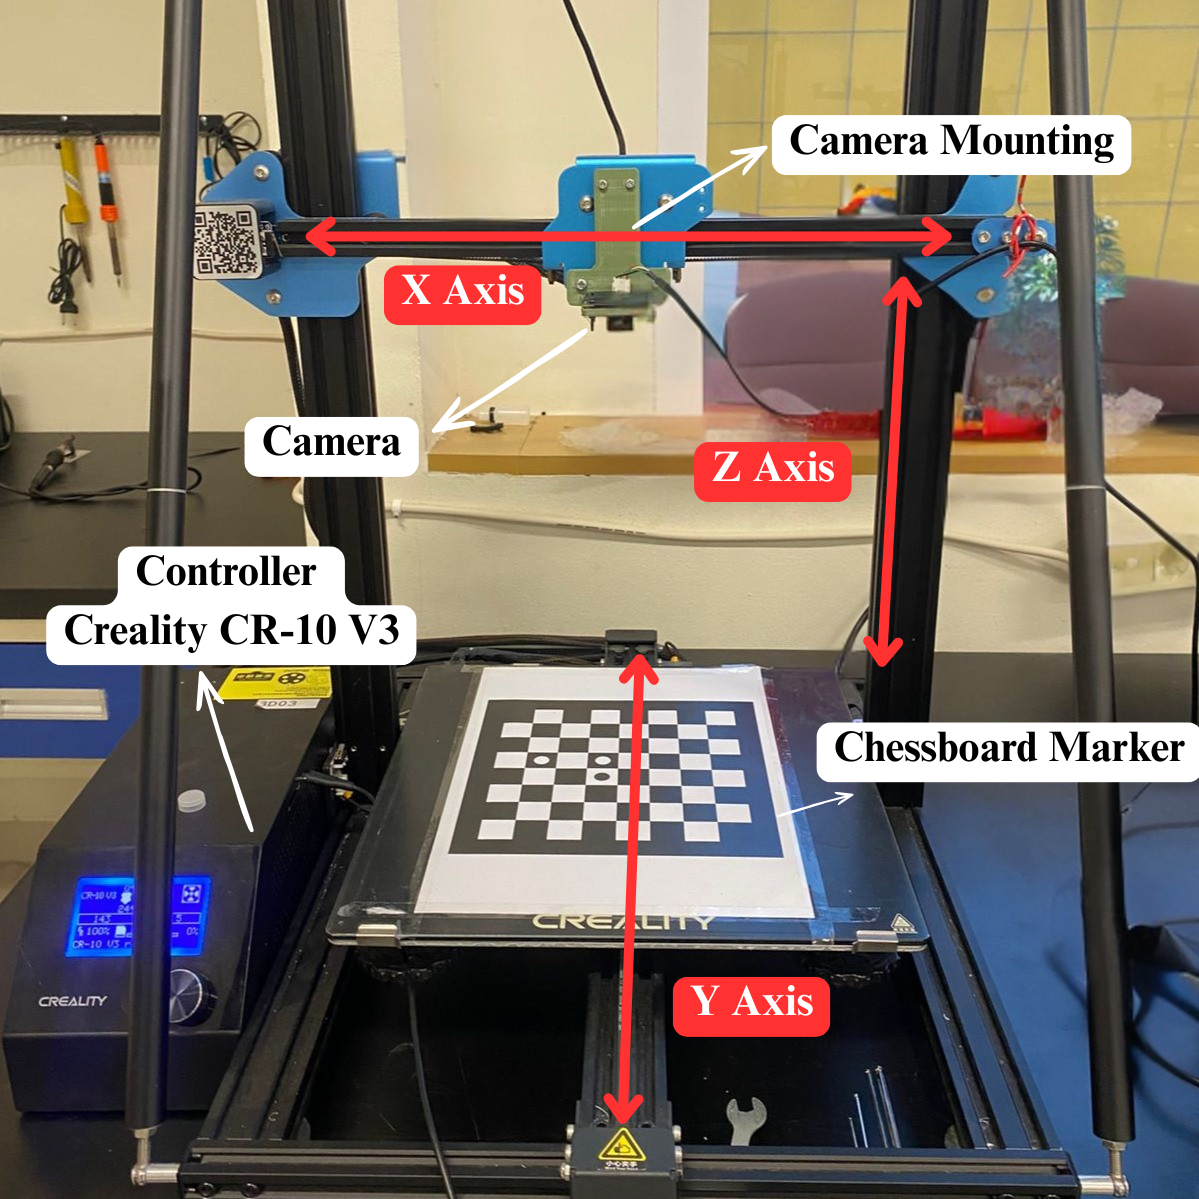
\includegraphics[width=0.8\linewidth]{images/setup.png}
    \caption{Experimental configuration of the
    camera-based virtual encoder.}
    \label{fig:setup}
\end{figure}

The marker contained $8\times8$ squares with
a nominal side length of 20~mm, providing
49 internal corners.
Three circular anchors with a radius of 5~mm
were included to support corner selection
and ordering.

Before displacement measurement, the camera was
calibrated using a dataset of ten board images
captured at different poses.
Corners were extracted and refined using
\eqref{eq:corner_objective} and
\eqref{eq:corner_solution}, then ordered using
the procedure in Section~\ref{homography}.
Images with a complete and successfully ordered
$7\times7$ grid were retained for calibration.
A representative result of feature extraction
and corner ordering is shown in
\figref{fig:Calib}.

\begin{figure}[htbp]
    \centering
    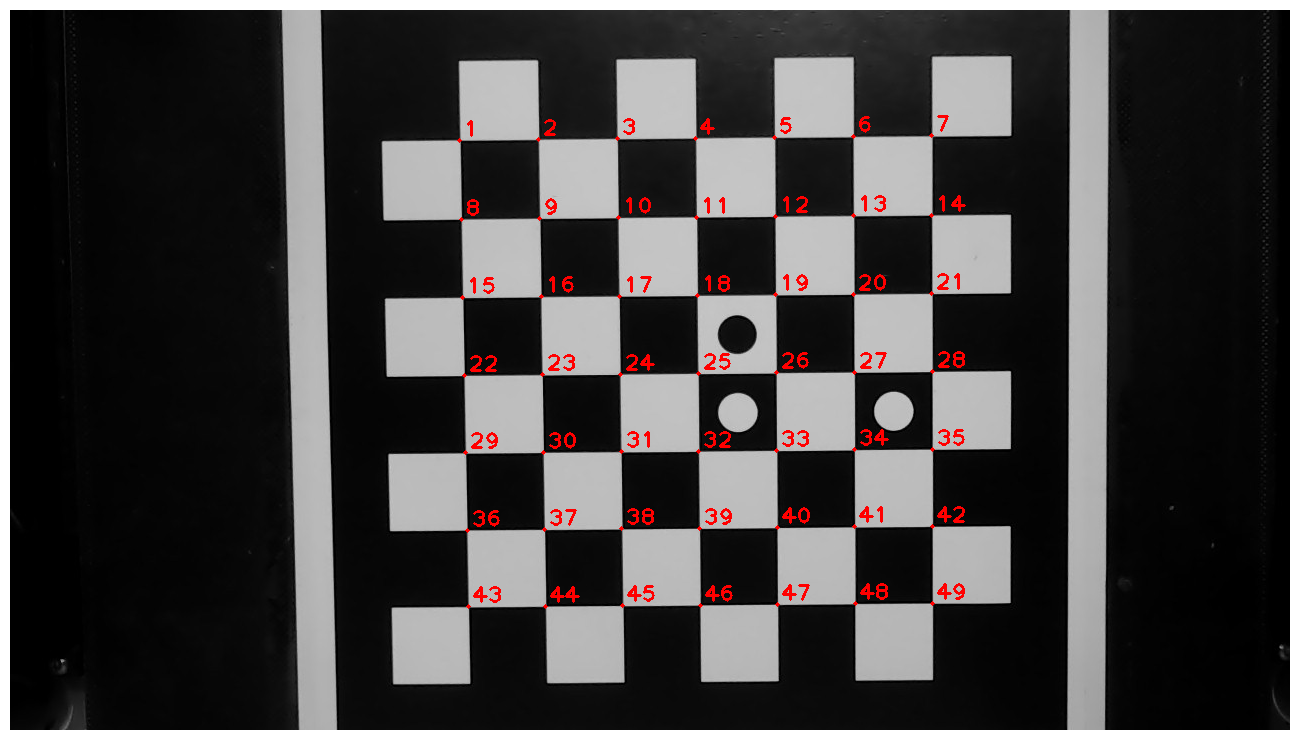
\includegraphics[width=0.8\linewidth]
    {images/result_after_corner_sorting.png}
    \caption{Detected and ordered chessboard corners
    in a representative calibration image.}
    \label{fig:Calib}
\end{figure}

The physical board coordinates were paired with
the detected image coordinates to estimate
the intrinsic matrix $K$, distortion coefficients
$D$, and board pose in each calibration image.
The parameters were obtained by minimizing
the sum of squared reprojection errors:
\begin{equation}
\label{eq:camera_calibration_objective}
\underset{K,D,\{R_i,t_i\}_{i=1}^{n}}
{\operatorname{minimize}}
\quad
\sum_{i=1}^{n}\sum_{j=1}^{m}
\left\|
\mathbf c_{ij}
-
\pi(\mathbf P_j;K,D,R_i,t_i)
\right\|_2^2,
\end{equation}
where $n$ is the number of retained calibration
images and $m=49$ is the number of corners
per image.
The vector $\mathbf c_{ij}$ denotes the detected
sub-pixel position of corner $j$ in image $i$.
The corresponding board coordinates $\mathbf P_j$
were expressed in millimeters.
The projection function $\pi(\cdot)$ follows
the camera model described in Section~\ref{sec:preliminaries}.

The estimated intrinsic matrix and distortion
coefficient vector were
\begin{equation}
\label{eq:intrinsic_matrix}
K=
\begin{bmatrix}
2314.64 & 0 & 637.08\\
0 & 2328.29 & 222.87\\
0 & 0 & 1
\end{bmatrix}
\end{equation}
and
\begin{equation}
\label{eq:distortion_coeffs}
D=
\begin{bmatrix}
-0.0561 & 0.9595 & 0.0001 & 0.0004 & -5.0330
\end{bmatrix},
\end{equation}
respectively.
The entries of $D$ correspond to
$[k_1,k_2,p_1,p_2,k_3]$, comprising three radial
and two tangential distortion coefficients.

Calibration quality was evaluated using
the overall reprojection RMSE:
\begin{equation}
\label{eq:camera_calibration_rmse}
e_{\mathrm{cal}}
=
\sqrt{
\frac{1}{nm}
\sum_{i=1}^{n}\sum_{j=1}^{m}
\left\|
\mathbf c_{ij}
-
\pi(\mathbf P_j;K,D,\hat R_i,\hat t_i)
\right\|_2^2
},
\end{equation}
where the projection was evaluated using
the estimated camera parameters and board poses.
The resulting RMSE was expressed in pixels.

The previous calibration results reported a mean
reprojection error of $0.1152$~pixels,
with a standard deviation of $0.0076$~pixels.
The calibrated $K$ and $D$ were subsequently
used by \textsc{ExtractPosition} in
Algorithm~\ref{alg:pose_extraction}.

\subsection{Measurement Procedure and Evaluation Metrics}

Measurement performance was evaluated through
reference displacement comparisons, single-axis
movement tests, and elliptical trajectory tests.
The motion tests were performed under baseline
and post-calibration conditions using the same
evaluation metrics.

For reference measurements, each axis was tested
separately against a mechanical dial gauge.
A commanded displacement of
$D_{\mathrm{cmd}}=0.5$~mm was selected within
the stated single-revolution range of 0.8~mm.
Each measurement cycle comprised initial,
forward, and reversal frames, as illustrated in
\figref{fig:positionextraction}.

The initial frame was captured at the starting
reference position.
The forward frame was captured after movement
by $+D_{\mathrm{cmd}}$, and the reversal frame
was captured after movement by
$-D_{\mathrm{cmd}}$ back toward the nominal
starting position.
Before the next cycle, an additional movement
of $-D_{\mathrm{cmd}}$ followed by
$+D_{\mathrm{cmd}}$ established a consistent
approach direction.
A new initial frame was then captured.

\begin{figure}[htbp]
    \centering
    \subfloat[]{
        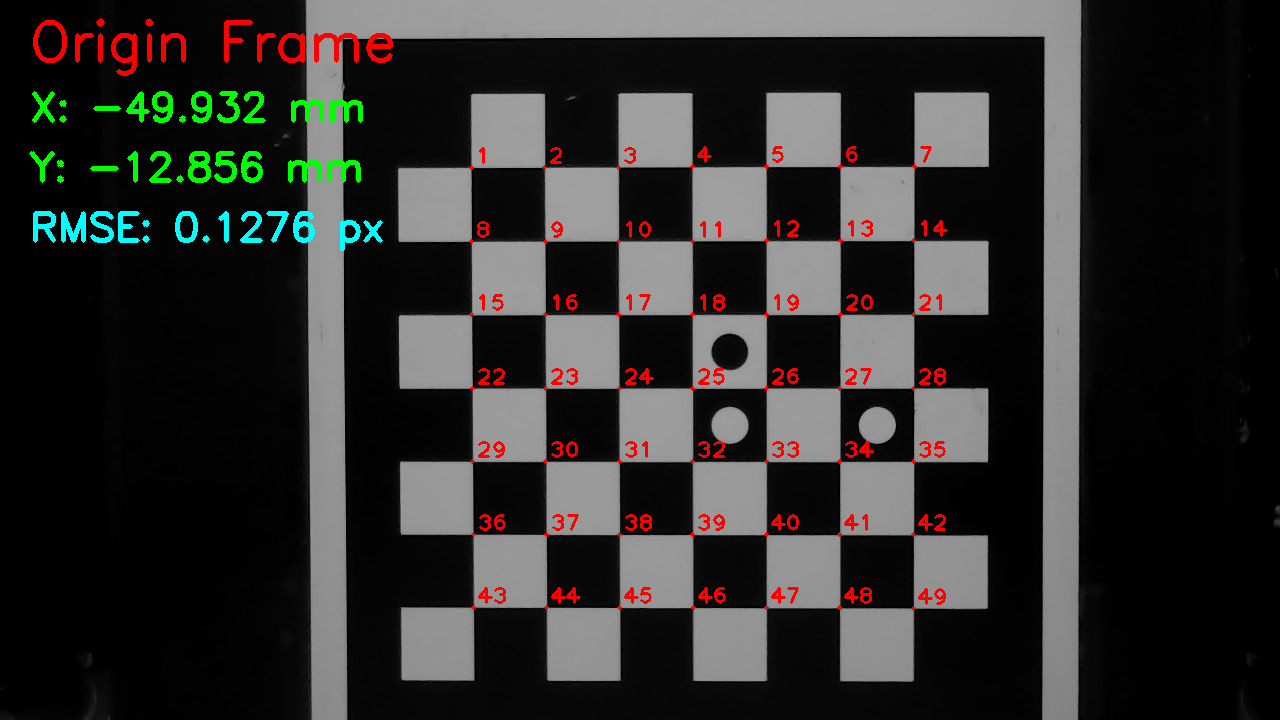
\includegraphics[width=0.75\linewidth]
        {images/visualisasi_ori.png}
        \label{fig:vis_ori}
    }

    \smallskip
    \subfloat[]{
        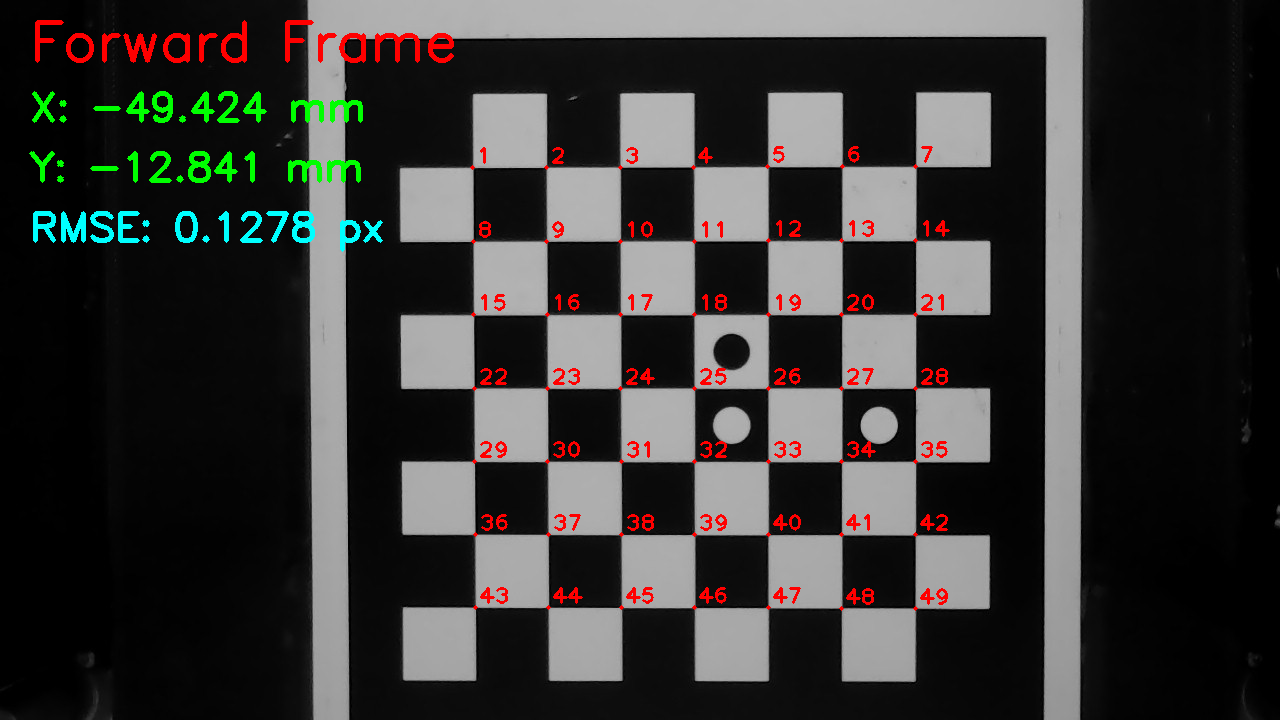
\includegraphics[width=0.75\linewidth]
        {images/visualisasi_fwd.png}
        \label{fig:vis_fwd}
    }

    \smallskip
    \subfloat[]{
        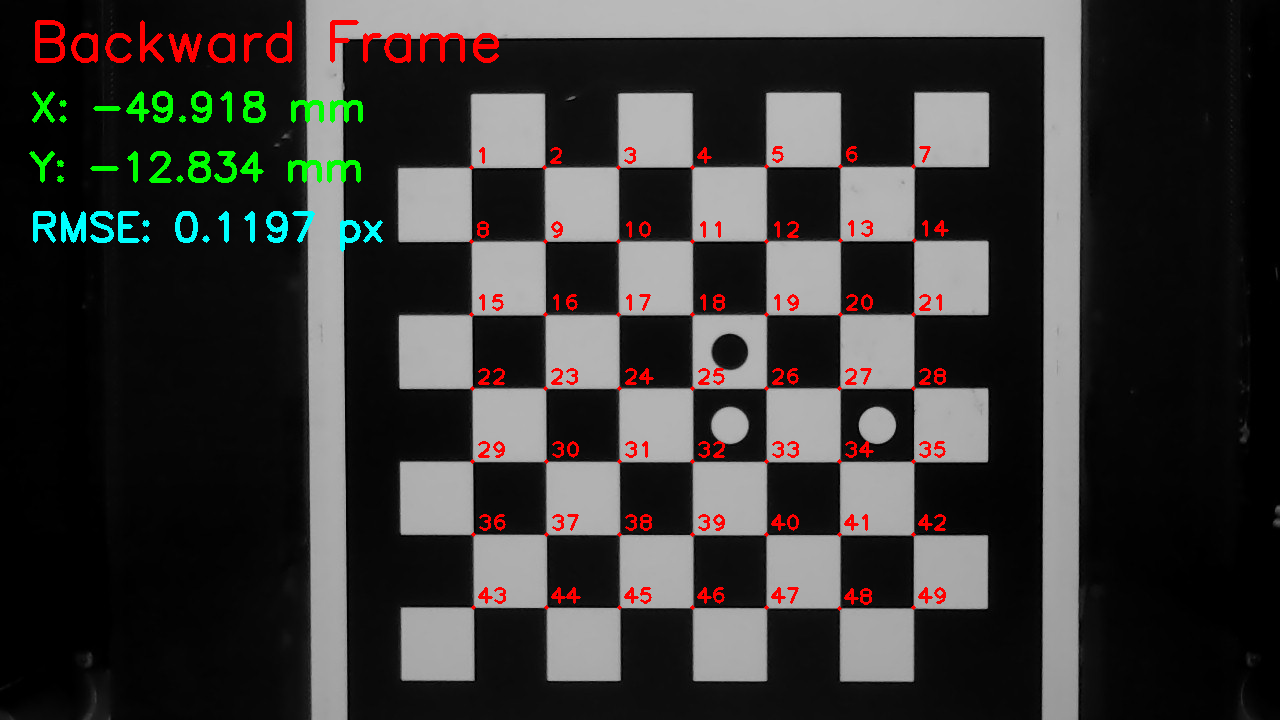
\includegraphics[width=0.75\linewidth]
        {images/visualisasi_bck.png}
        \label{fig:vis_bck}
    }
    \caption{Representative position extraction
    results for one active axis:
    (a) initial frame,
    (b) forward frame, and
    (c) reversal frame.}
    \label{fig:positionextraction}
\end{figure}

Positions were extracted using
\textsc{ExtractPosition} in
Algorithm~\ref{alg:pose_extraction}.
Only image triplets with valid position estimates
and reprojection errors satisfying
$\epsilon_i\le\epsilon_{\mathrm{th}}$
for all three frames were retained.
Encoder displacements relative to the initial
position were compared with the corresponding
dial gauge readings.

For each movement condition, the mean absolute
measurement discrepancy was calculated as
\begin{equation}
\label{eq:encoder_reference_mae}
e_{\mathrm{MAE}}
=
\frac{1}{N_{\mathrm{valid}}}
\sum_{i=1}^{N_{\mathrm{valid}}}
\left|
d_{\mathrm{enc},i}-d_{\mathrm{dial},i}
\right|,
\end{equation}
where $N_{\mathrm{valid}}$ is the number of
accepted measurement cycles.
The quantities $d_{\mathrm{enc},i}$ and
$d_{\mathrm{dial},i}$ denote the encoder and
reference displacement readouts, respectively.
Both readouts were expressed in the same length
unit and used the same direction convention.

Single-axis motion was evaluated using the same
initial, forward, and reversal sequence.
The signed positioning deviation was calculated as
\[
e_{\mathrm{pos},i}=d_i-D_{\mathrm{cmd}},
\]
where $d_i$ is the measured active-axis
displacement.
Reversal-related lost motion and cross-axis
drift were evaluated using
\eqref{eq:kinematic_error_metrics}.
The calibration parameters were obtained using
Algorithm~\ref{alg:kompensasi}.
The same movement sequence and error metrics
were used before and after compensation.

Coordinated X--Y motion was evaluated along
the commanded elliptical path shown in
\figref{fig:circexam}.
The printer executed the path through G-code,
and video frames were processed using
\textsc{ExtractPosition}.
Invalid position estimates and frames with
reprojection errors exceeding
$\epsilon_{\mathrm{th}}$ were excluded.

\begin{figure}[htbp]
    \centering
    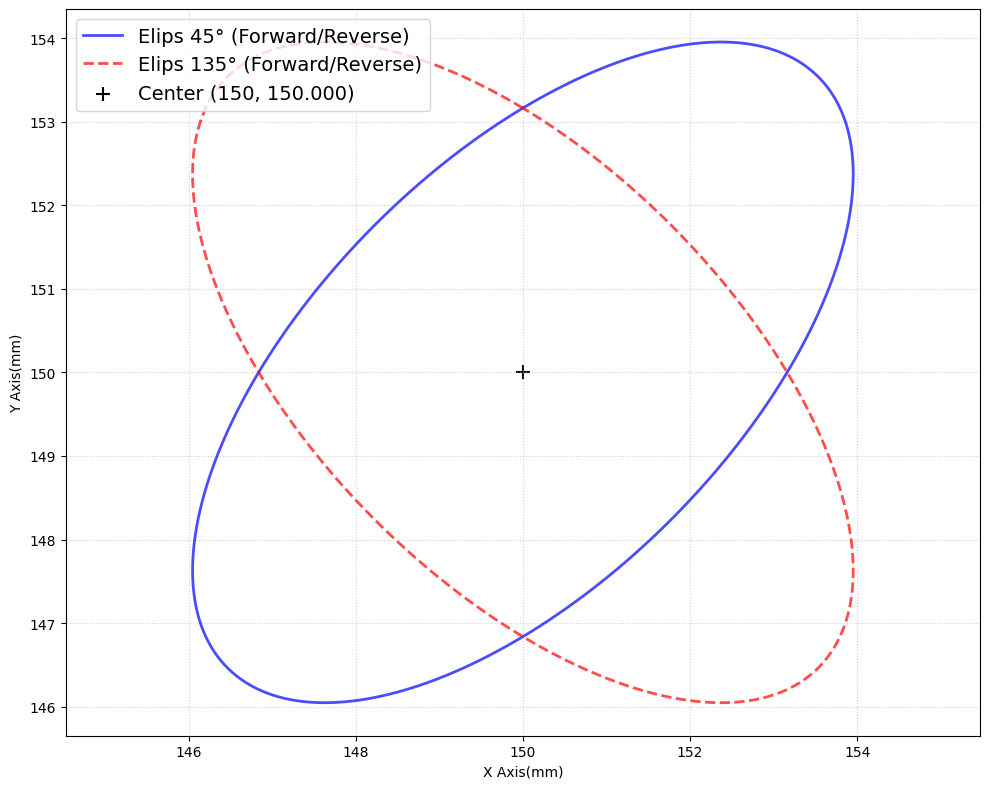
\includegraphics[width=0.8\linewidth]
    {images/circularmovement.png}
    \caption{Commanded elliptical trajectory
    for coordinated X--Y motion evaluation.}
    \label{fig:circexam}
\end{figure}

For each trial, the measured trajectory was
translated to align its first accepted position
with the reference starting point:
\begin{equation}
\label{eq:trajectory_origin_alignment}
\tilde{\mathbf p}_k
=
\mathbf p_k-\mathbf p_0+\mathbf r_0,
\end{equation}
where $\mathbf p_k$ is the extracted position,
$\mathbf p_0$ is the first accepted position,
and $\mathbf r_0$ is the reference starting point.
Measured and reference positions were expressed
in a common coordinate frame and in millimeters.

Each aligned position was associated with
the nearest sampled reference point:
\begin{equation}
\label{eq:trajectory_nearest_reference}
\begin{aligned}
j_k^{*}
&=
\underset{j}{\arg\min}
\left\|
\tilde{\mathbf p}_k-\mathbf r_j
\right\|_2,\\
\mathbf e_k
&=
\tilde{\mathbf p}_k-\mathbf r_{j_k^{*}},
\end{aligned}
\end{equation}
where $\mathbf r_j$ is a sampled reference point
and $\mathbf e_k=[e_{x,k},e_{y,k}]^{\mathsf T}$
is the geometric deviation.
A KD-tree was used for nearest-neighbor search.

For $L$ accepted positions, the trajectory
deviation metrics were calculated as
\begin{equation}
\label{eq:trajectory_deviation_rmse}
\begin{aligned}
E_x
&=
10^3
\sqrt{\frac{1}{L}
\sum_{k=1}^{L}e_{x,k}^{2}},\\
E_y
&=
10^3
\sqrt{\frac{1}{L}
\sum_{k=1}^{L}e_{y,k}^{2}},\\
E_{\mathrm{tot}}
&=
10^3
\sqrt{\frac{1}{L}
\sum_{k=1}^{L}\|\mathbf e_k\|_2^{2}}.
\end{aligned}
\end{equation}
The factor $10^3$ converts millimeters
to micrometers.
These metrics quantify geometric deviation
from the sampled reference path.
They do not quantify motion delay or
time-synchronized tracking error.
Trial-wise RMSE values were summarized across
repeated tests and compared between baseline
and post-calibration conditions.

\subsection{Measurement Discrepancy and Uncertainty}

The virtual encoder displacement readouts were compared
with the dial gauge measurements using
\eqref{eq:encoder_reference_mae}.
The measurement comparison for the forward and
reversal conditions is shown in
\figref{fig:position_comparison}.
Evaluated with \eqref{eq:encoder_reference_mae}, the mean
absolute discrepancies were $4.96~\mu\text{m}$ for the
X-axis and $7.81~\mu\text{m}$ for the Y-axis.
The corresponding direction-dependent mean offsets were
$3.8~\mu\text{m}$ forward and $3.3~\mu\text{m}$ backward
on the X-axis, and $8.5~\mu\text{m}$ forward and
$4.0~\mu\text{m}$ backward on the Y-axis. Because these
offsets reverse sign with the travel direction, they
partially cancel when averaged over both directions,
giving net offsets of $-0.2~\mu\text{m}$ and
$+2.3~\mu\text{m}$, respectively.
These values described agreement with the reference
readings over the tested 0.5~mm displacement range.

\begin{figure}[htbp]
    \centering
    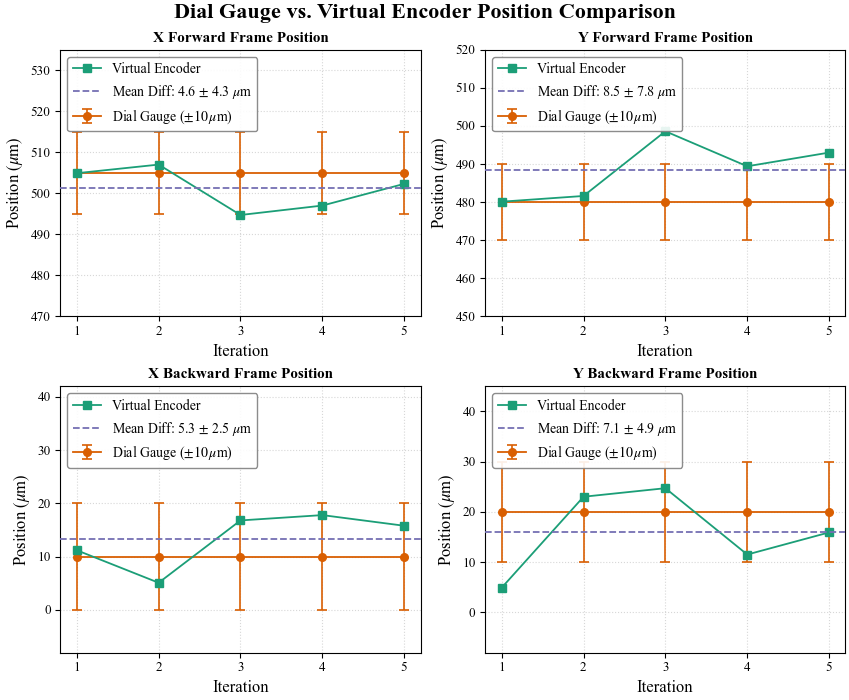
\includegraphics[width=\linewidth]
    {images/1_4_position_comparison_combined.png}
    \caption{Comparison of dial gauge and virtual
    encoder position readouts for the X and Y axes
    under forward and reversal conditions.}
    \label{fig:position_comparison}
\end{figure}

Stationary measurements were used to characterize
fluctuations in the position readout, as shown in
\figref{fig:Noise}.
The mean absolute readout deviations were
$2.58~\mu\text{m}$ and $4.97~\mu\text{m}$ for the
X and Y axes, and the standard deviations of the repeated
stationary readout were $2.63~\mu\text{m}$ and
$3.44~\mu\text{m}$, respectively.
These results characterized measurement stability
under stationary conditions.

\begin{figure}[htbp]
    \centering
    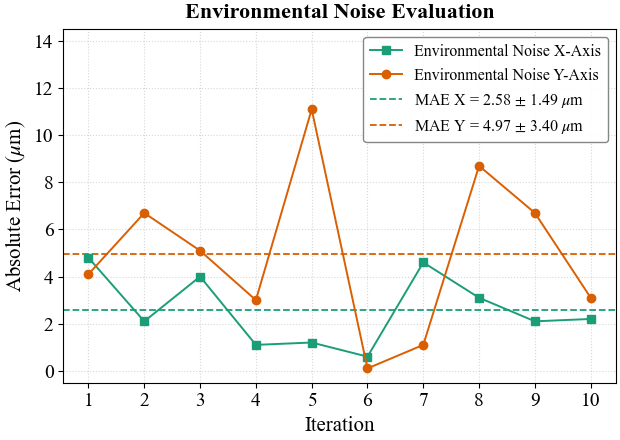
\includegraphics[width=0.8\linewidth]
    {images/Noise_Lingkungan.png}
    \caption{Stationary position readout fluctuations
    for the X and Y axes.}
    \label{fig:Noise}
\end{figure}

An uncertainty budget was formulated using
the ISO/IEC Guide 98-3 (GUM) framework.
Assuming uncorrelated contributions expressed
in displacement units, the combined standard
uncertainty was calculated as
\begin{equation}
\label{eq:gum_uc}
u_c
=
\sqrt{
u_A^2+
u_{\mathrm{dial}}^2
}.
\end{equation}
The Type A repeatability contribution was evaluated from
$N=5$ repeated measurements per travel direction as
\[
u_A=\frac{\sigma}{\sqrt{N}},
\]
where $\sigma$ is the sample standard deviation of the
repeated displacement measurements within a travel
direction, pooled over the forward and reversal conditions.
The stationary readout dispersion reported above is of the
same order as this term and originates from the same readout
noise; it was therefore characterized separately instead of
being added as an independent contribution, so that the same
dispersion is not counted twice. The sub-pixel reprojection
residual was likewise retained as an indicator of model-fit
quality rather than as an uncertainty contribution, because
it is already reflected in the dispersion of the measured
displacement.

For a reference instrument error interval
$[-a,a]$ with a rectangular distribution,
the standard uncertainty was calculated as
\[
u_{\mathrm{dial}}=\frac{a}{\sqrt{3}}.
\]
The quantity $a$ denotes the half-width of the assumed
reference error interval and is distinct from
the dial gauge resolution.
Using $a=10~\mu\text{m}$ gave
$u_{\mathrm{dial}}=5.77~\mu\text{m}$.

The expanded uncertainty was calculated using
a coverage factor $k=2$:
\begin{equation}
\label{eq:gum_expanded}
U=k u_c=2u_c.
\end{equation}
This coverage factor corresponds to approximately
95\% coverage when the distributional and
effective degrees-of-freedom assumptions are satisfied.
The individual uncertainty contributions and the
reported combined and expanded uncertainties
are summarized in Table~\ref{tab:uncertainty_budget}.

\begin{table}[htbp]
    \centering
    \caption{Measurement Uncertainty Budget
    for the Virtual Encoder System}
    \label{tab:uncertainty_budget}
    \scriptsize
    \setlength{\tabcolsep}{2.5pt}
    \renewcommand{\arraystretch}{1.2}

    \begin{tabularx}{\linewidth}{@{} L c c c c @{}}
        \toprule
        \textbf{Source of Uncertainty} &
        \textbf{Symbol} &
        \textbf{Distribution} &
        \textbf{X ($\mu$m)} &
        \textbf{Y ($\mu$m)} \\
        \midrule

        Measurement Repeatability (Type A) &
        $u_A$ &
        Normal &
        2.34 &
        3.57 \\

        Reference Dial Gauge Tolerance &
        $u_{\mathrm{dial}}$ &
        Rectangular &
        5.77 &
        5.77 \\
        \midrule

        \textbf{Combined Standard Uncertainty} &
        $u_c$ &
        --- &
        \textbf{6.23} &
        \textbf{6.79} \\

        \textbf{Expanded Uncertainty} &
        $U$ &
        --- &
        \textbf{12.46} &
        \textbf{13.57} \\
        \bottomrule
    \end{tabularx}

    \smallskip
    \parbox{\linewidth}{\scriptsize
    Repeatability was evaluated using $N=5$ repeated
    measurements per travel direction. The stationary
    readout dispersion is reported separately and is not
    added to the budget, so that the same readout noise is
    not counted twice. The sub-pixel reprojection residual
    is reported as a model-fit indicator, not as an
    uncertainty contribution. Expanded uncertainty used a
    coverage factor $k=2$.}

\end{table}

The dial gauge contribution was the largest individual
component in the reported budget.
The mean absolute encoder--reference discrepancies
were smaller than the expanded uncertainties.
However, this comparison did not establish coverage
for every individual measurement or independently
demonstrate absolute accuracy below
$7~\mu\text{m}$.

\subsection{Linear-Axis Calibration Results}

Baseline measurements showed mean positioning errors
of $46.3~\mu\text{m}$ and $55.0~\mu\text{m}$
for the X and Y axes, respectively.
The corresponding reversal-related errors were
$12.4~\mu\text{m}$ and $24.4~\mu\text{m}$.
Single-axis movements also exhibited cross-axis drift,
with reported drift angles of $-0.5344^\circ$
for X displacement during Y motion and
$0.5171^\circ$ for Y displacement during X motion.
These angles described motion relative to the
measurement coordinate frame and did not independently
establish mechanical axis non-orthogonality.

The calibration parameters were refined using
Algorithm~\ref{alg:kompensasi}.
Figures~\ref{fig:x_axis_iter} and
\ref{fig:y_axis_iter} compare positioning,
cross-axis drift, and reversal-related errors
across ten evaluation iterations for the X and Y
axes, respectively, under baseline and calibrated
conditions.

\begin{figure}[htbp]
    \centering
    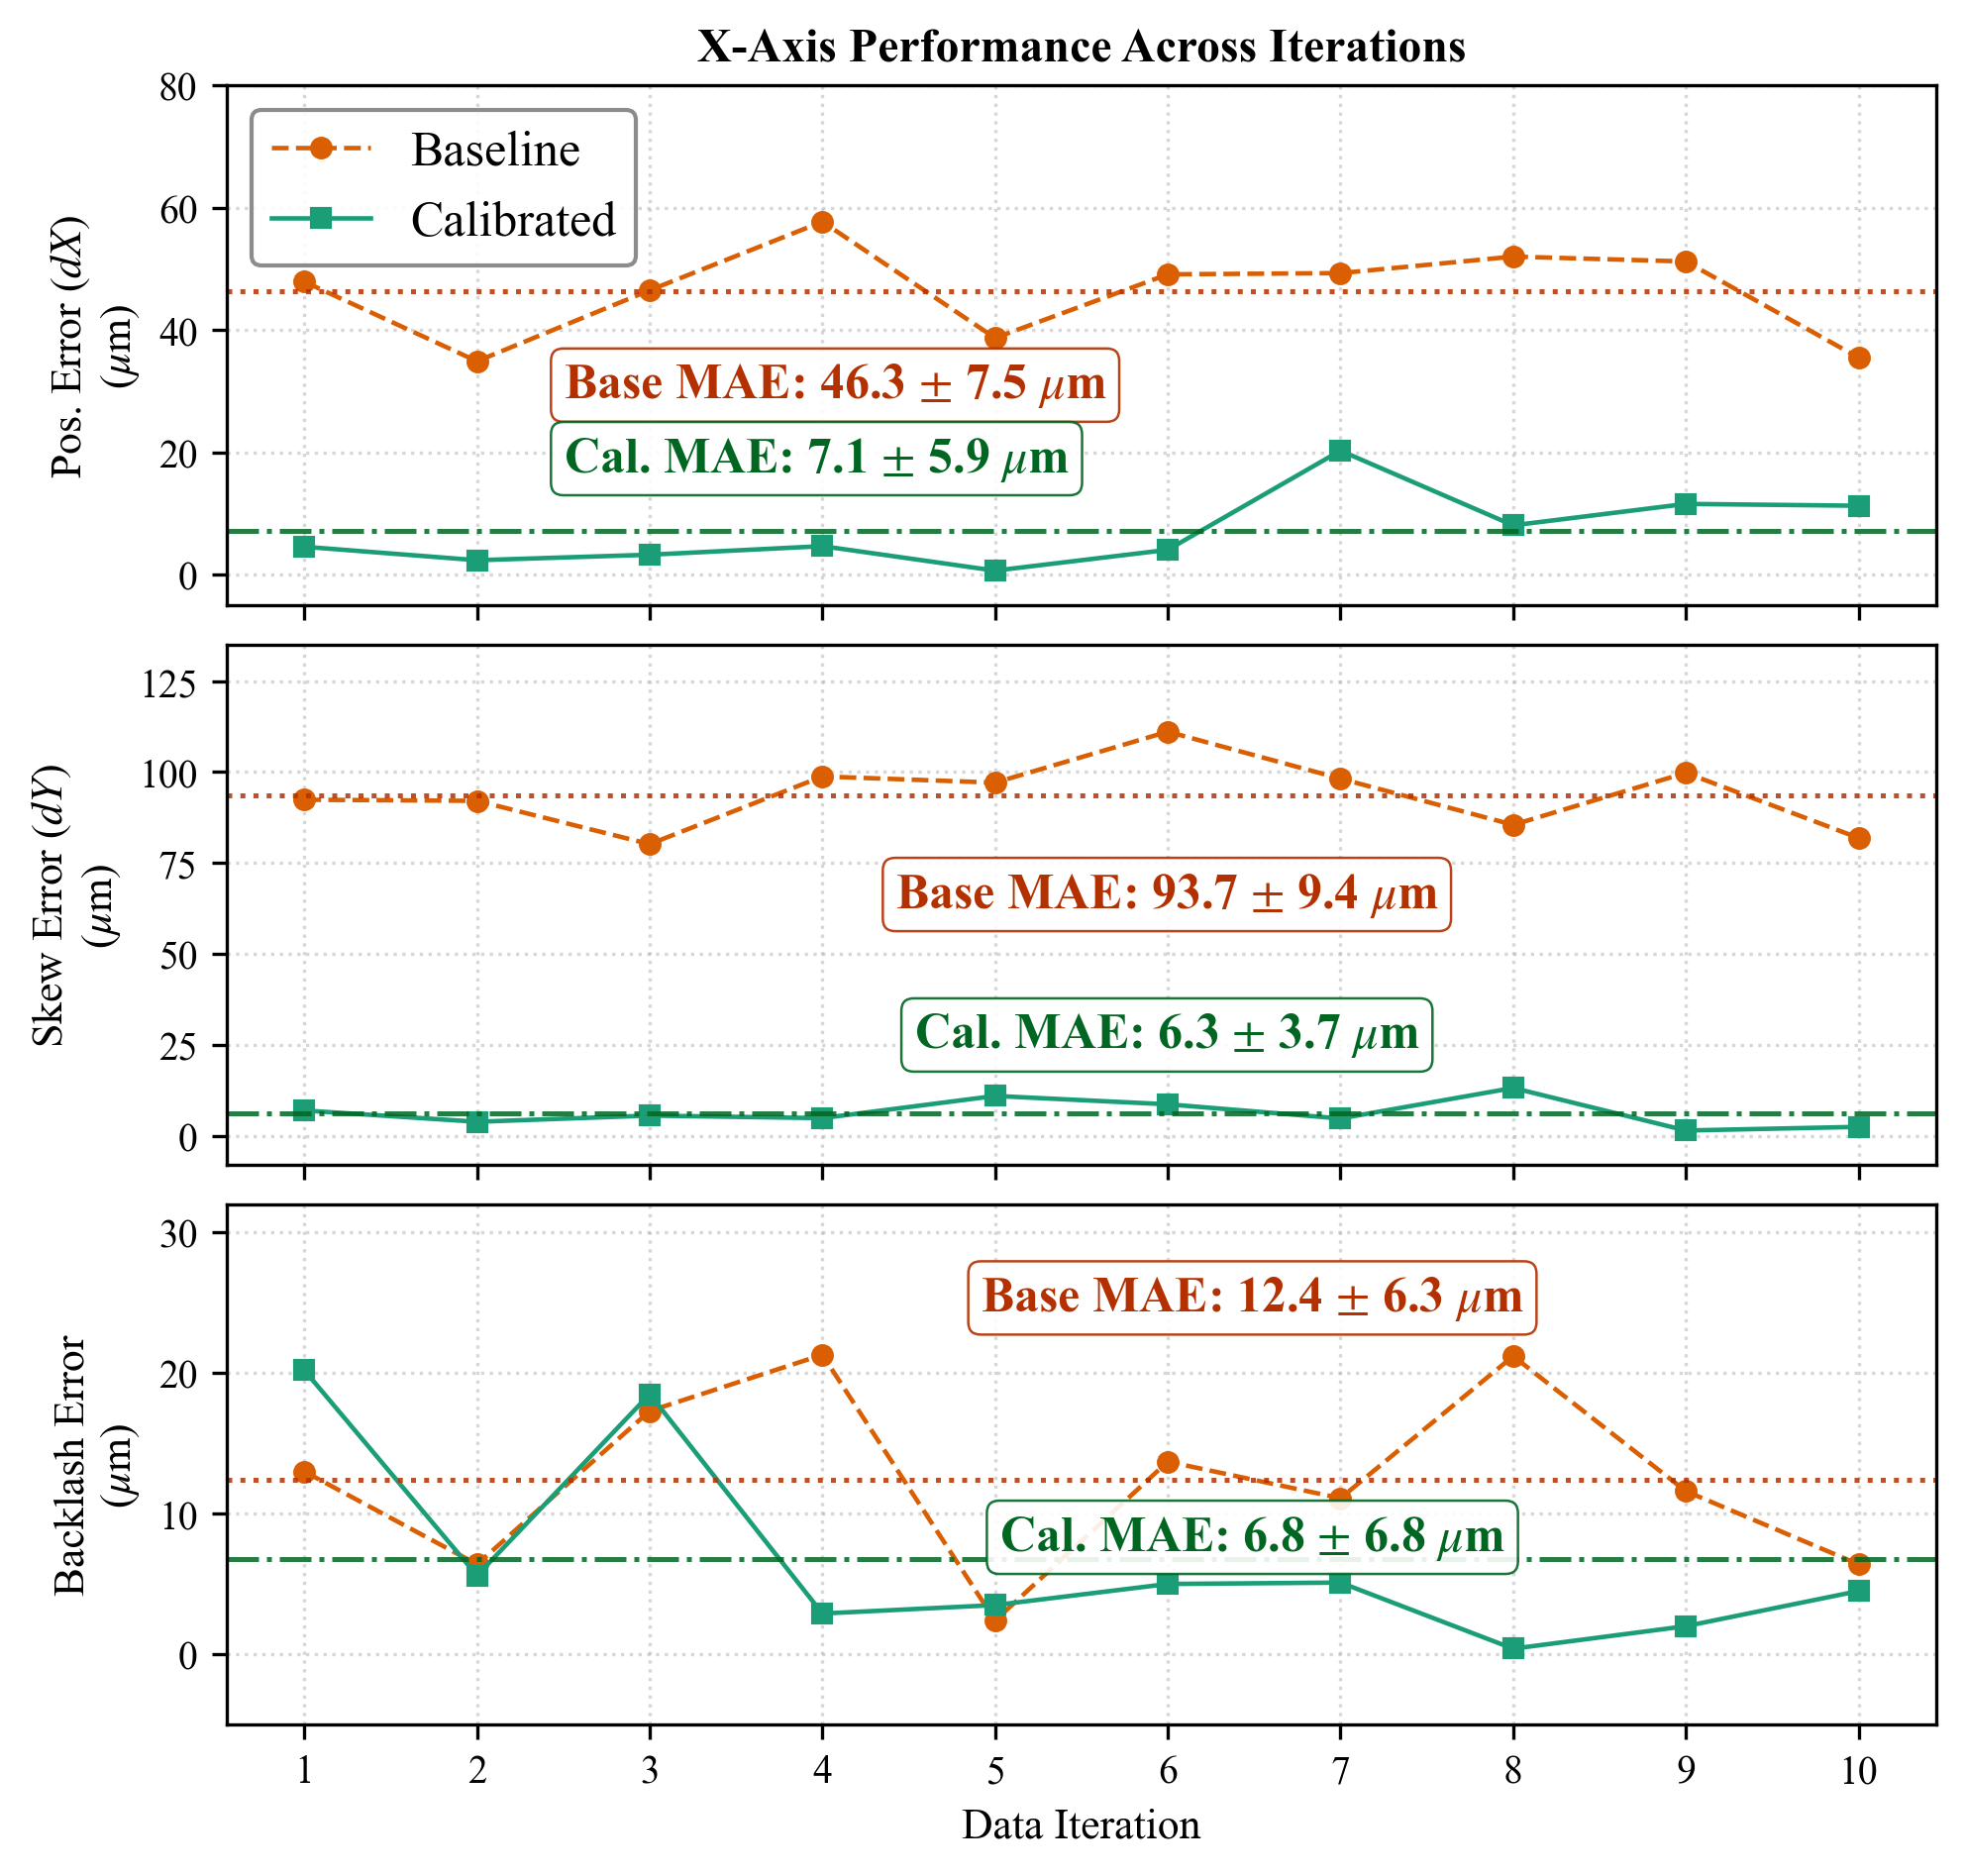
\includegraphics[width=\linewidth]
    {images/x_axis_iterations.png}
    \caption{X-axis positioning, cross-axis drift,
    and reversal-related errors across ten evaluation
    iterations under baseline and calibrated conditions.}
    \label{fig:x_axis_iter}
\end{figure}

\begin{figure}[htbp]
    \centering
    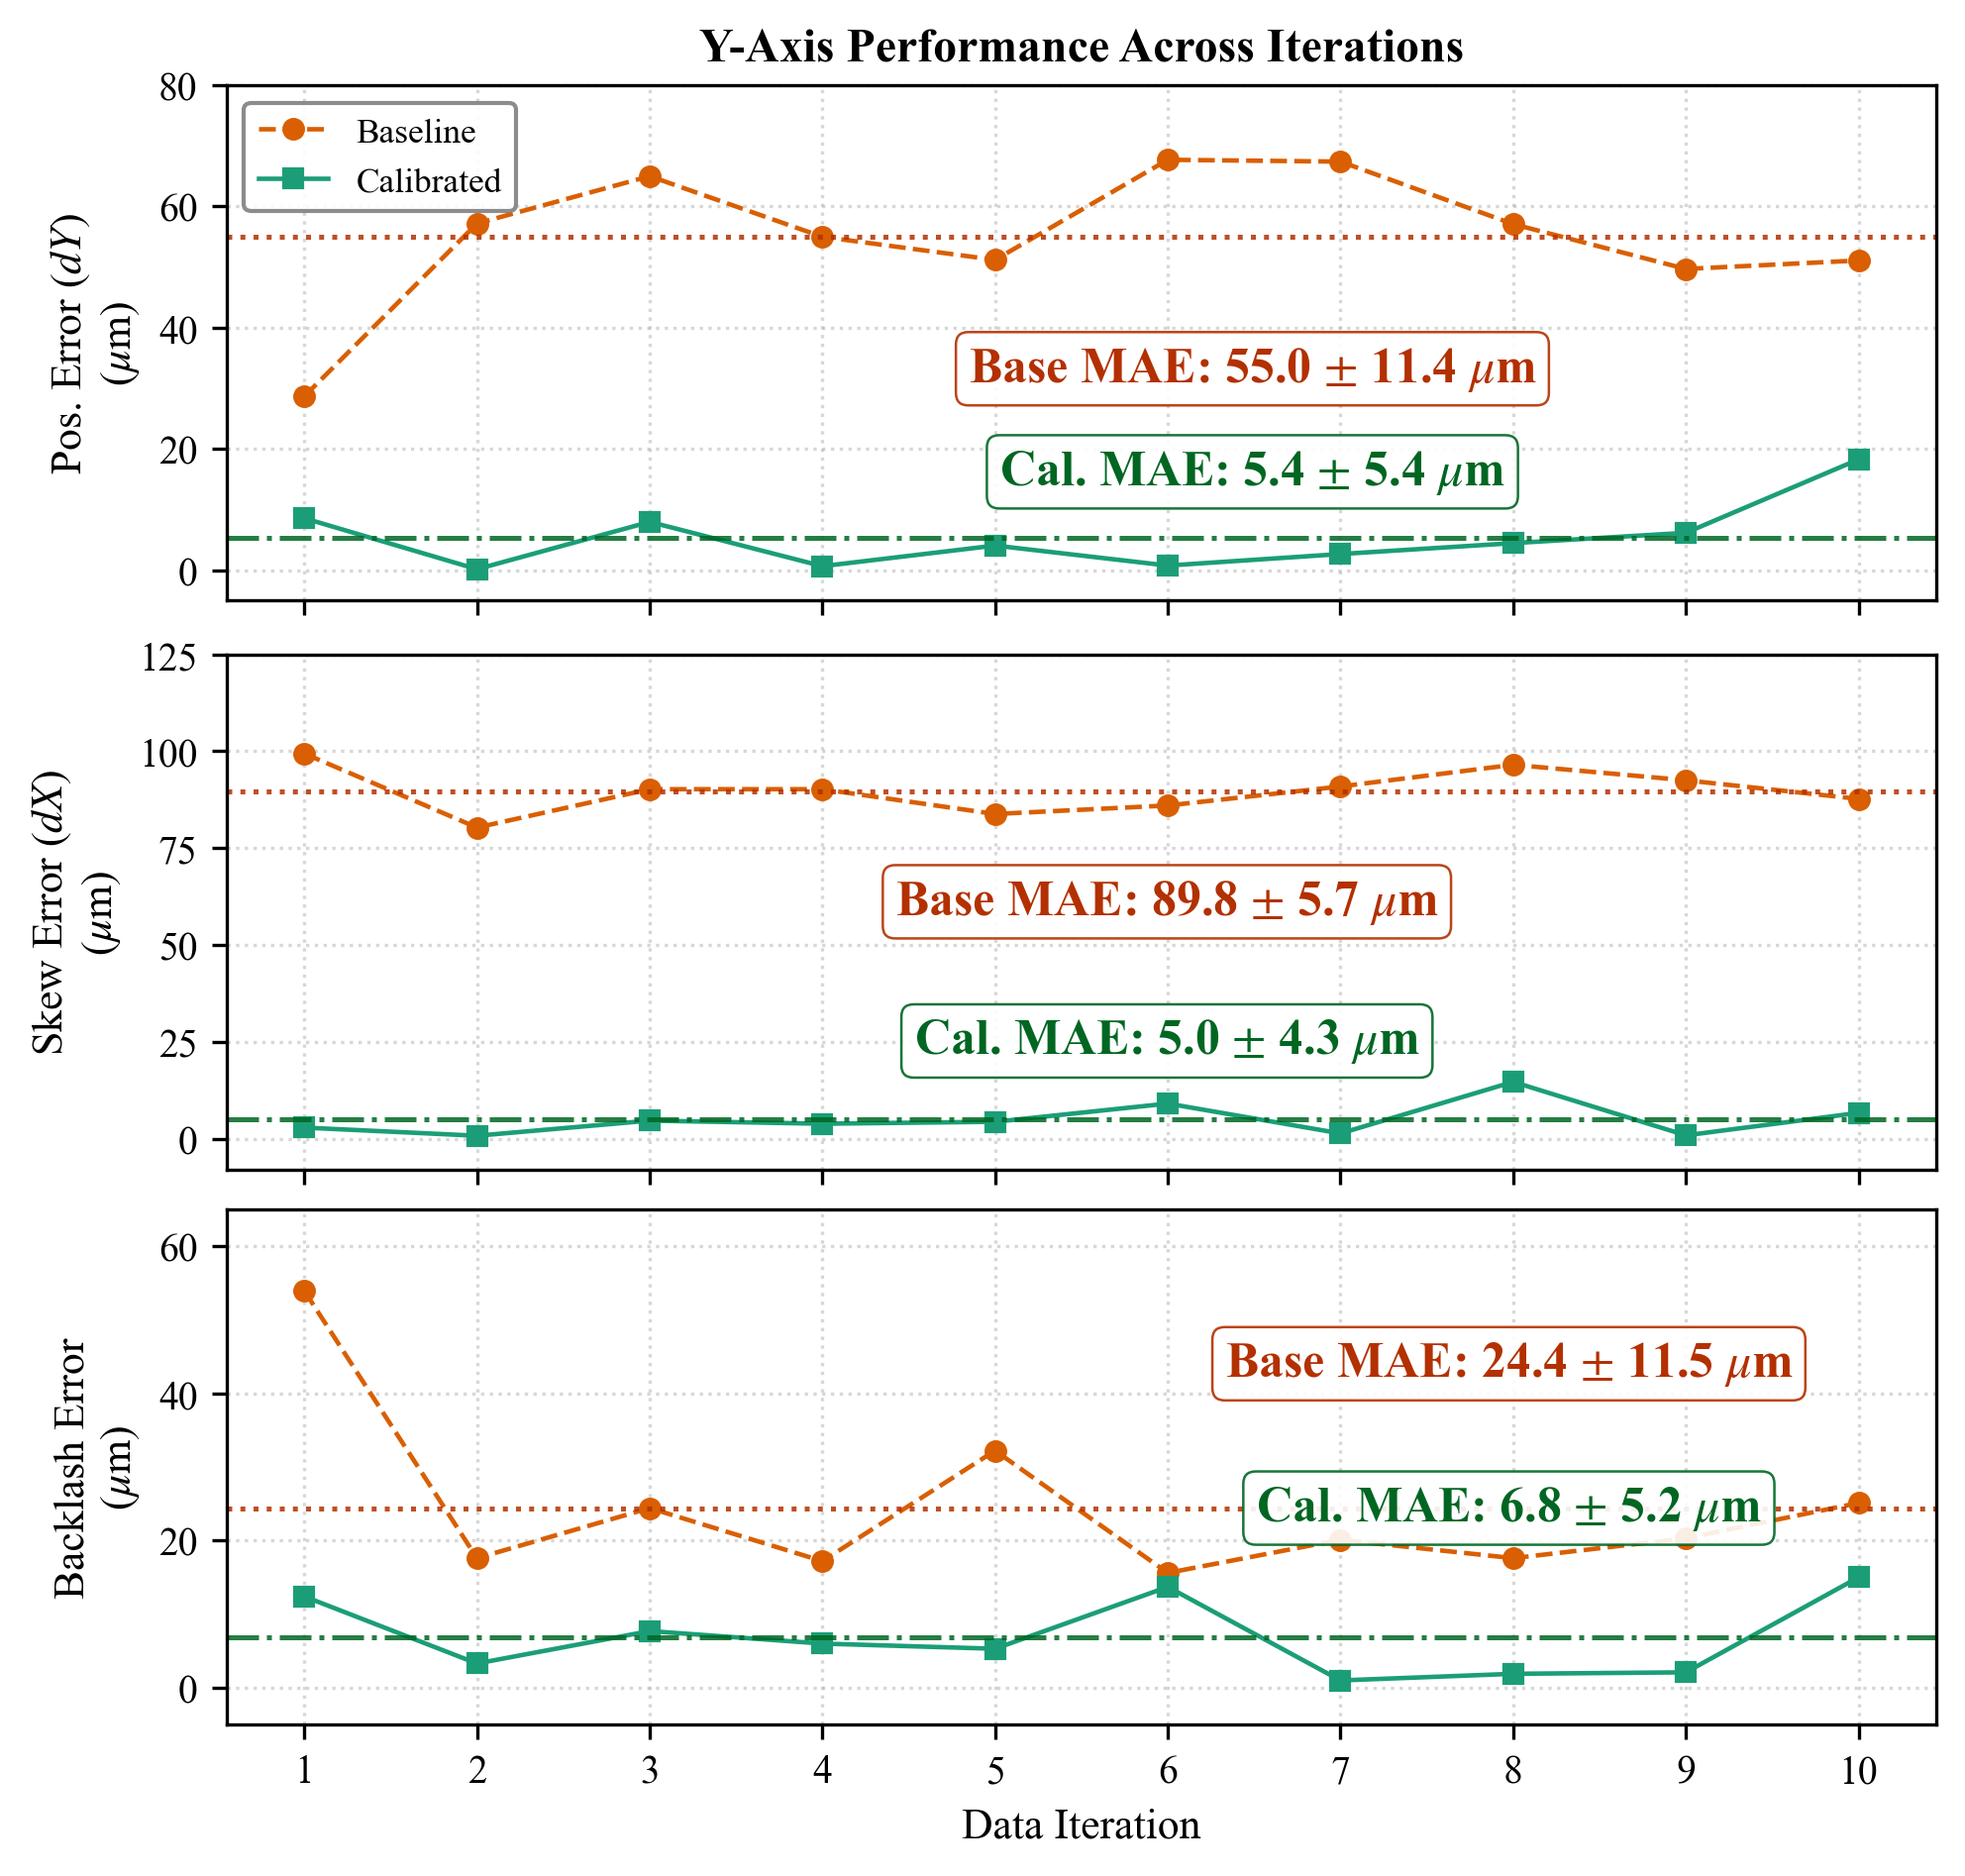
\includegraphics[width=\linewidth]
    {images/y_axis_iterations.png}
    \caption{Y-axis positioning, cross-axis drift,
    and reversal-related errors across ten evaluation
    iterations under baseline and calibrated conditions.}
    \label{fig:y_axis_iter}
\end{figure}

Table~\ref{tab:parameter_final_kalibrasi} lists
the final steps-per-millimeter settings,
lost-motion compensation values, and cross-axis
correction slopes.
These values represented the applied compensation
parameters rather than the residual errors
after calibration.

\begin{table}[htbp]
    \centering
    \caption{Final Linear-Axis Calibration Parameters}
    \label{tab:parameter_final_kalibrasi}
    \footnotesize
    \setlength{\tabcolsep}{4pt}
    \renewcommand{\arraystretch}{1.15}

    \begin{tabularx}{\linewidth}{@{} l L r @{}}
        \toprule
        \textbf{Parameter} &
        \textbf{Description} &
        \textbf{Final Value} \\
        \midrule

        \texttt{STEPX} &
        X-axis steps-per-millimeter setting &
        79.72 steps/mm \\

        \texttt{STEPY} &
        Y-axis steps-per-millimeter setting &
        80.40 steps/mm \\
        \midrule

        \texttt{BACKLASH\_X} &
        X-axis lost-motion compensation &
        $13.3~\mu\text{m}$ \\

        \texttt{BACKLASH\_Y} &
        Y-axis lost-motion compensation &
        $31.4~\mu\text{m}$ \\
        \midrule

        \texttt{SKEW\_X\_ON\_Y} &
        Parasitic X-drift during Y motion &
        $-9.2~\mu\text{m/mm}$ \\

        \texttt{SKEW\_Y\_ON\_X} &
        Parasitic Y-drift during X motion &
        $9.213~\mu\text{m/mm}$ \\
        \bottomrule
    \end{tabularx}

    \smallskip
    \parbox{\linewidth}{\footnotesize
    Cross-axis values denote the identified drift
    slopes used in
    \eqref{eq:cross_axis_compensation}.
    The listed parameters are compensation settings,
    not residual errors after calibration.}
\end{table}

The mean absolute errors and percentage reductions
are summarized in \figref{fig:maesum}.
After compensation, the X-axis positioning error
decreased by 84.6\% to
$7.1\pm5.9~\mu\text{m}$.
Its cross-axis drift and reversal-related errors
decreased by 93.3\% and 45.6\%, reaching
$6.3\pm3.7~\mu\text{m}$ and
$6.8\pm6.8~\mu\text{m}$, respectively.
For the Y-axis, the positioning error decreased
by 90.2\% to $5.4\pm5.4~\mu\text{m}$.
Cross-axis drift decreased by 94.5\% to
$5.0\pm4.3~\mu\text{m}$, while the
reversal-related error decreased by 72.0\%
to $6.8\pm5.2~\mu\text{m}$.

\begin{figure}[htbp]
    \centering
    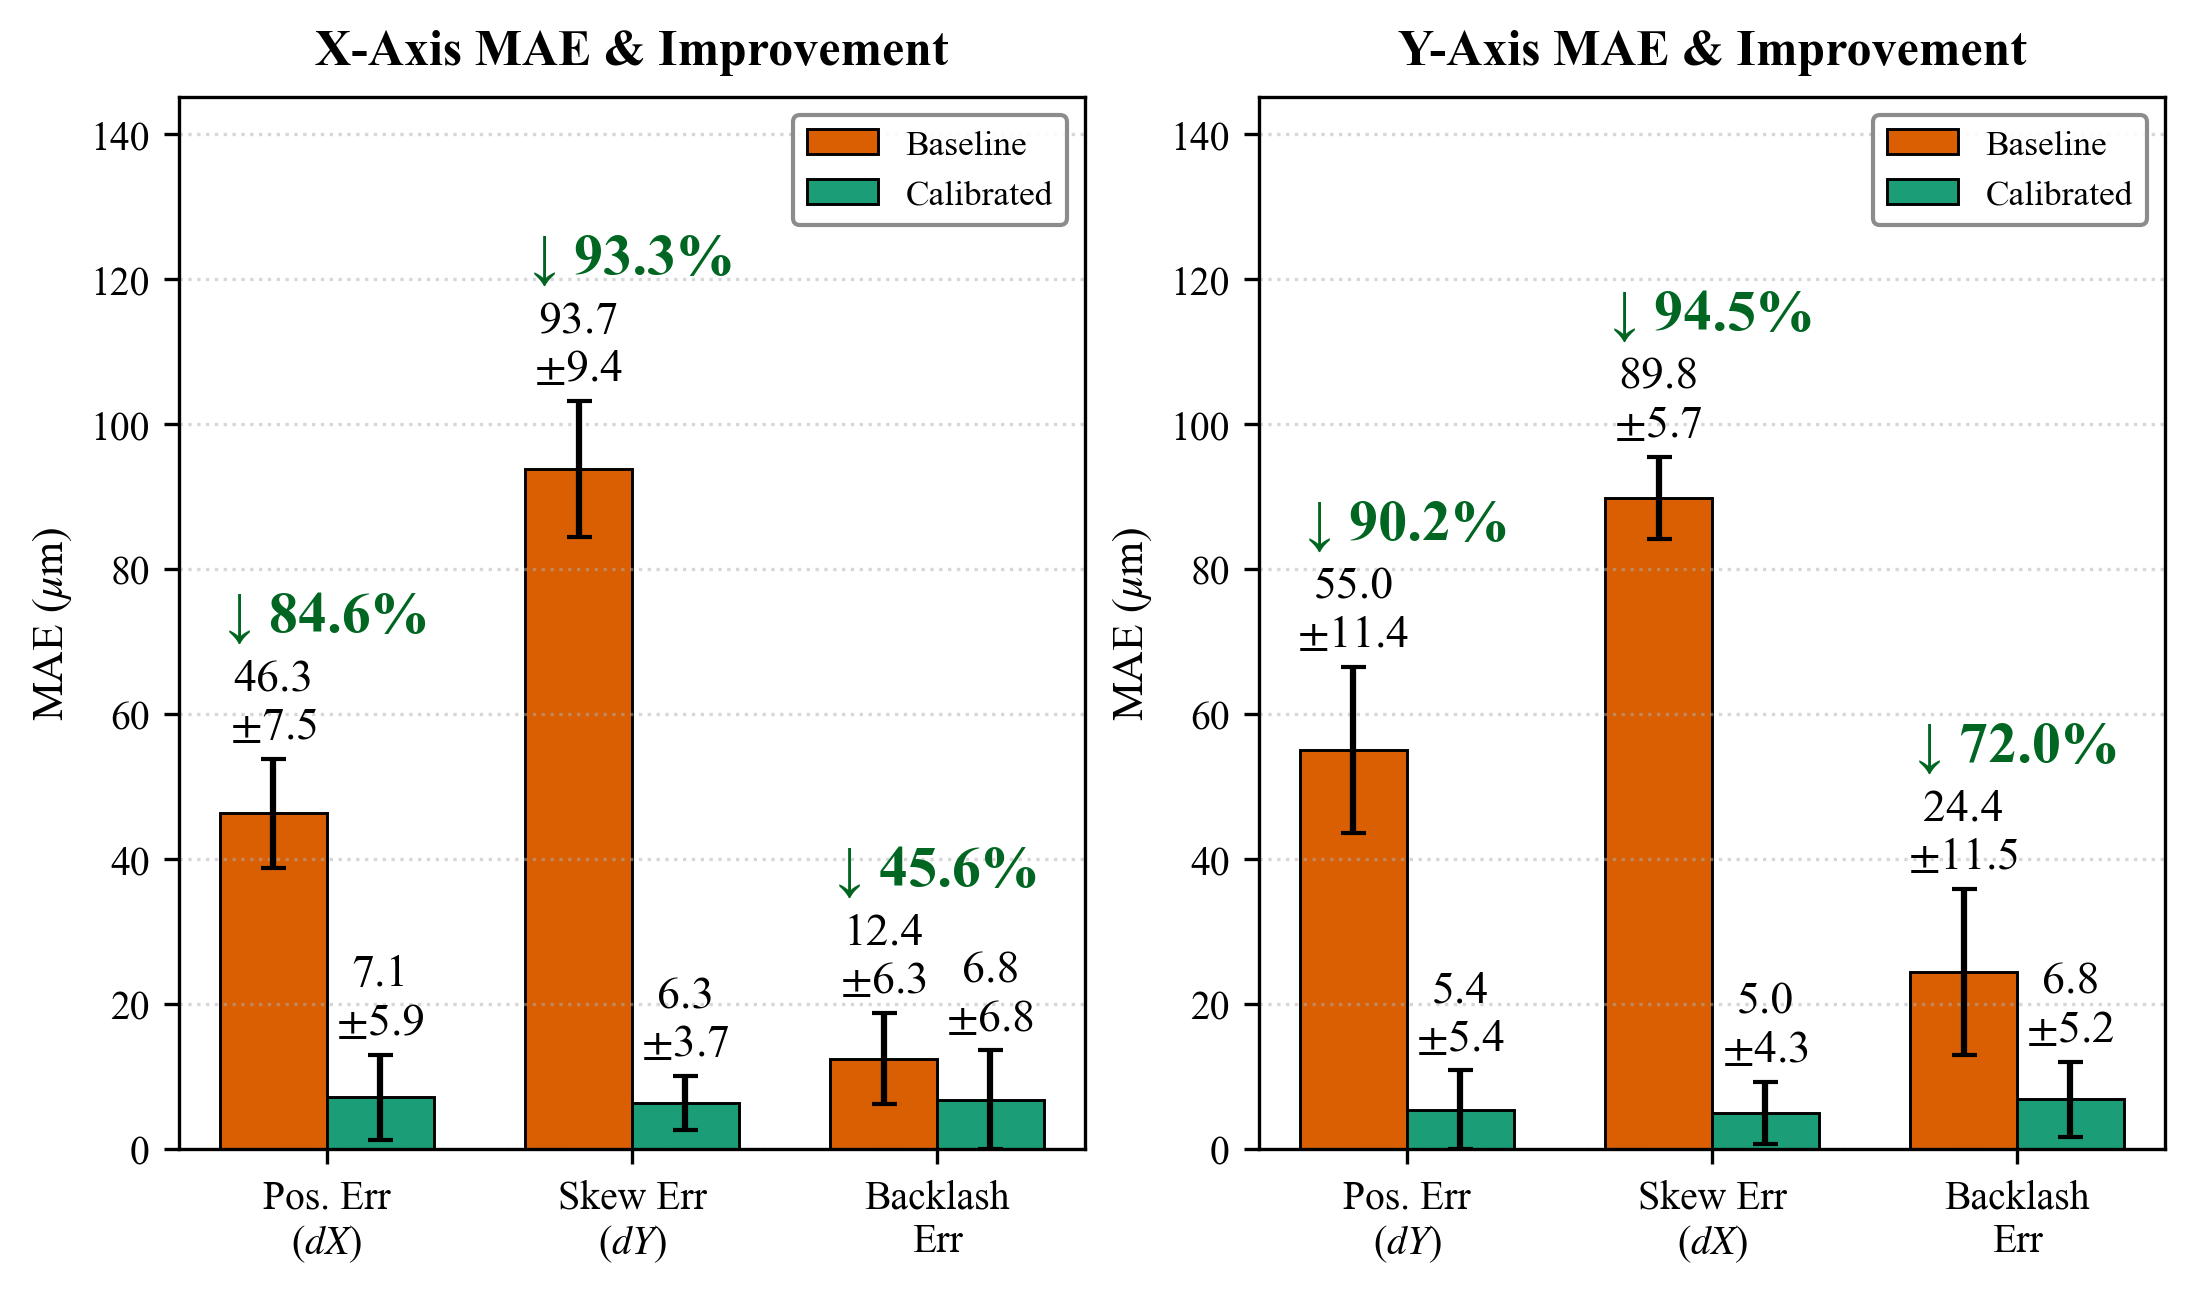
\includegraphics[width=\linewidth]
    {images/mae_summary.png}
    \caption{Mean absolute errors and percentage
    reductions for positioning, cross-axis drift,
    and reversal-related error on the X and Y axes.}
    \label{fig:maesum}
\end{figure}

The results showed reductions in all evaluated
linear-motion error components.
Positioning and cross-axis drift exhibited larger
percentage reductions than reversal-related error.
The remaining deviations were interpreted alongside
the measurement uncertainty reported in the preceding
subsection. These results supported improved motion
performance under the tested conditions.

\subsection{Elliptical Trajectory Results}

The elliptical trajectory tests evaluated coordinated
X--Y motion under baseline and post-calibration
conditions. Geometric deviations from the commanded
reference path were calculated using
\eqref{eq:trajectory_deviation_rmse}.
The baseline total trajectory RMSE was
$100.9\pm7.4~\mu\text{m}$.

After calibration, the X-axis trajectory RMSE
decreased by 55.25\% to
$34.42\pm1.70~\mu\text{m}$, while the Y-axis
RMSE decreased by 52.91\% to
$30.75\pm1.37~\mu\text{m}$.
The total trajectory RMSE decreased by 54.24\%
to $46.17\pm1.77~\mu\text{m}$.
These results showed that the calibration parameters
obtained from single-axis measurements also reduced
geometric deviations during coordinated motion.

The remaining trajectory deviations were greater
than the residual errors observed in the linear-axis
tests. This difference indicated that improved
single-axis positioning did not eliminate deviations
during continuous multi-axis movement.
The trajectory results therefore complemented
the linear-axis evaluation by assessing performance
under coordinated motion.

Because the evaluation associated each measured
position with the nearest sampled reference point,
the reported RMSE values characterized geometric
path deviation. They did not quantify motion delay
or time-synchronized tracking error.


\section{Conclusion}
\label{conclusion}
This study developed a low-cost, machine vision-based virtual encoder for XY-axis calibration of a 3D printer using a planar chessboard marker, EDLines-based corner extraction, and iterative PnP pose estimation. Measurement discrepancies relative to the dial gauge were $4.96~\mu\text{m}$ and $7.81~\mu\text{m}$ for the X and Y axes, respectively. After calibration, positioning errors decreased by 84.6\% on the X-axis and 90.2\% on the Y-axis, reaching $7.1 \pm 5.9~\mu\text{m}$ and $5.4 \pm 5.4~\mu\text{m}$, respectively. Cross-axis drift and reversal-related errors also decreased. The total elliptical trajectory deviation decreased by 54.24\%, from $100.9~\mu\text{m}$ to $46.17 \pm 1.77~\mu\text{m}$ RMSE. These results demonstrated that vision-based measurement and software compensation improved the printer's motion performance under the tested conditions with a measurement hardware cost below USD~30.

% --- BIBLIOGRAPHY ---
\bibliographystyle{IEEEtran}
\bibliography{IEEEabrv,Bibliography}

\end{document}